\documentclass[10pt]{article}

\usepackage[margin=0.8in]{geometry}

\setlength{\parindent}{0pt}

\usepackage{listings}
\lstset{
    language=R,
    basicstyle=\ttfamily
}
\usepackage{biblatex}
\usepackage{subcaption} 
\usepackage{mlmodern}
\usepackage{xcolor}
\usepackage[]{amsthm}
\usepackage[]{amsmath}
\usepackage[]{amsfonts}
\usepackage{bm}
\usepackage{graphicx}
\usepackage{makecell}
\usepackage{booktabs}
\usepackage{rotating}
\usepackage{multirow}
\graphicspath{ {./Images/} }
\DeclareMathOperator*{\argmin}{argmin} 

\newtheorem{theorem}{Theorem}
\newtheorem{corollary}{Corollary}[theorem] % Use theorem counter as `parent`
\newtheorem{lemma}{Lemma}


\definecolor{codegreen}{rgb}{0,0.6,0}
\definecolor{codegray}{rgb}{0.5,0.5,0.5}
\definecolor{codepurple}{rgb}{0.58,0,0.82}
\definecolor{backcolour}{rgb}{0.95,0.95,0.92}

\lstdefinestyle{mystyle}{
    backgroundcolor=\color{white},   
    commentstyle=\color{codegreen},
    keywordstyle=\color{magenta},
    numberstyle=\tiny\color{codegray},
    stringstyle=\color{codepurple},
    basicstyle=\ttfamily\footnotesize,
    breakatwhitespace=false,         
    breaklines=true,                 
    captionpos=b,                    
    keepspaces=true,                 
    numbers=left,                    
    numbersep=5pt,                  
    showspaces=false,                
    showstringspaces=false,
    showtabs=false,                  
    tabsize=2
}

\lstset{style=mystyle}


\title{\vspace{-1cm}Beauty Beyond Ratings: Unveiling the Sentiment and Secrets of Beauty Products Using Ulta's Online Text Data}
\author{Andrew Mashhadi $\vert$ Final Project $\vert$ Stats 425}
\date{}

\begin{document}

\maketitle

\section{Introduction}

For decades, Ulta Beauty has retained its position as one of the most popular chains of beauty stores in the United States. Ulta Beauty carries both high-end and low-end cosmetics, fragrances, nail products, bath and body products, beauty tools, and haircare products. In recent years, however, Ulta Beauty has conducted much of its business online. Almost all the products are readily available and purchased through the official Ulta website. In addition to the convenience of ordering products online, customers may also evaluate specific products through online ratings and share their product experiences through online reviews. Ratings and reviews, in combination with product descriptions, present a plethora of text data that may serve useful for brands looking to conduct market research on their products.  

\

More than 600 independent brands are sold through Ulta. In general, many brands rely on performance metrics and consumer opinions provided by social media, advertisements, or even surveys to determine the success of their individual products. Brands would benefit greatly from a comprehensive report of their product's performance metrics on an online retailer such as Ulta. Unfortunately, most brands are not provided with the detailed metrics or overall sentiment of their corresponding products from Ulta. Using modern text-mining methods with the reviews, ratings, and descriptions of each product's associated webpage, we may be able to extract more information from the Ulta website than a traditional survey, and would certainly be able to save cost and time by leveraging the automation of our analyses. In this paper, we embark on a journey to accomplish several distinctive goals. With an exploratory analysis approach, our primary objectives are as follows:

\begin{enumerate}
    \item Uncover Customer Sentiment | We extract and analyze customer sentiment for individual products, brands, and product categories, providing insights into customer perceptions.
    \item Revealing Word Trends | By examining frequently occurring words and employing \textit{tf-idf} scores, we delve into product descriptions to uncover word patterns that correlate with sentiment expressed in reviews and ratings.
    \item Discovering Commonalities | Through topic modeling, we aim to identify underlying themes and commonalities across diverse brands, offering a holistic view of the beauty industry.
    \item Contrasting Term Frequencies | We compare and contrast relative term frequencies within the derived ``topics'' and among a few selected popular makeup brands, enabling valuable comparisons and highlighting unique brand characteristics.
\end{enumerate}

By pursuing these goals, we aim to shed light on the intricate dynamics and trends within Ulta's online beauty store, providing valuable insights for both customers and brands alike. In addition to our exploratory analysis, we embark on a more focused modeling endeavor to formally characterize the intricate relationships within the Ulta data. With a specific modeling approach, we aim to achieve the following goals:

\begin{enumerate}
    \item Predicting Average Star Ratings | We endeavor to create a robust model capable of predicting the average star rating of a product based on the corresponding customer reviews. This predictive framework will provide valuable insights into the factors influencing customer satisfaction.
    \item Unveiling the Price-Sentiment Nexus | By modeling the relationship between product price and customer sentiment, we aim to unravel the intricate interplay between these two crucial aspects. This analysis will provide valuable insights into the dynamics between price points and customer perceptions.
    \item Leveraging Textual Descriptions | Our ambition is to develop a classification model that can predict whether a product is highly rated solely based on the textual content of its description. This text-driven model will enable efficient evaluation and assessment of products, independent of external factors.
\end{enumerate}

Through these focused modeling approaches, we aim to enhance our understanding of the Ulta dataset, unravel hidden patterns, and unlock invaluable insights for both consumers and businesses in the beauty industry.

\section{Data Collection \& Software Used}

Using the \texttt{rvest} library in \texttt{R}, we scraped Ulta's online text data from each brand and each product. That is, we iterated through every product from each brand available on the Ulta website, and then collected the following data for each associated product:

\begin{itemize}
    \item \texttt{brand\_name}: the brand name associated with the product
    \item \texttt{product\_id}: the unique product identifier
    \item \texttt{product\_name}: the product name (may not be unique)
    \item \texttt{product\_class}: the category of the product (haircare, nail products, etc.)
    \item \texttt{description\_text}: the product description text data
    \item \texttt{review\_text}: the customer reviews for the product
    \item \texttt{product\_rating}: the average customer star rating for the product (0-5)
    \item \texttt{product\_price}: the product's associated price
\end{itemize}

Approximately 15,247 unique products were scraped from the Ulta website. To prevent a lengthy web-scraping process, we randomly sampled $n_i = 5$ customer reviews per product. If products had less than $n_i < 5$ reviews, we collected \textit{all} of the customer reviews for that product. We should note that the restriction of at most 5 reviews per product was also shown to prevent extended runtime delays in our analyses. In total, over 61,457 customer reviews were used in our study.

\

For each brand, the collected data was stored locally in CSV format. Depending on the type of analysis, files may have been concatenated within \texttt{R} and grouped by brand or by product category. Each analysis conducted read the data files into \texttt{R} and often involved text-mining libraries such as \texttt{tidytext}, \texttt{tm}, and \texttt{topicmodels}, in addition to other common machine-learning and graphics libraries. 

\section{Exploratory Analysis}

As mentioned above, we have a set of goals that were achieved through an exploratory analysis approach. Prior to conducting the analysis, we applied techniques covered in class to clean the text data, which involved removing numbers, punctuation, and English stop-words, as well as eliminating duplicate reviews. We now discuss the results of each analysis in detail.

\subsection{Uncovering Customer Sentiment}

To begin, we used the numerical sentiment scores from the \textit{AFINN Sentiment Lexicon} to extract each review's overall sentiment score. To give equal weight to each review for a specific product, we classified each review as either ``positive'' or ``negative'' based on the total (sum) sentiment score, and then used the proportion of positive reviews as the final sentiment score for the individual product.

\

Figure (1) presents word-clouds generated from reviews with low star ratings (left) and high star ratings (right). While there are common words appearing in both plots, it is evident that the word cloud associated with high star ratings reflects a positive theme, whereas the word cloud associated with low star ratings exhibits a negative theme. To validate the accuracy of our predicted sentiments, we compared our sentiment scores with the normalized average star ratings for each product.

\begin{figure}[ht!]
    \hspace*{0em}
    \centering 
    \subcaptionbox{Star-Rating $<1.5$}{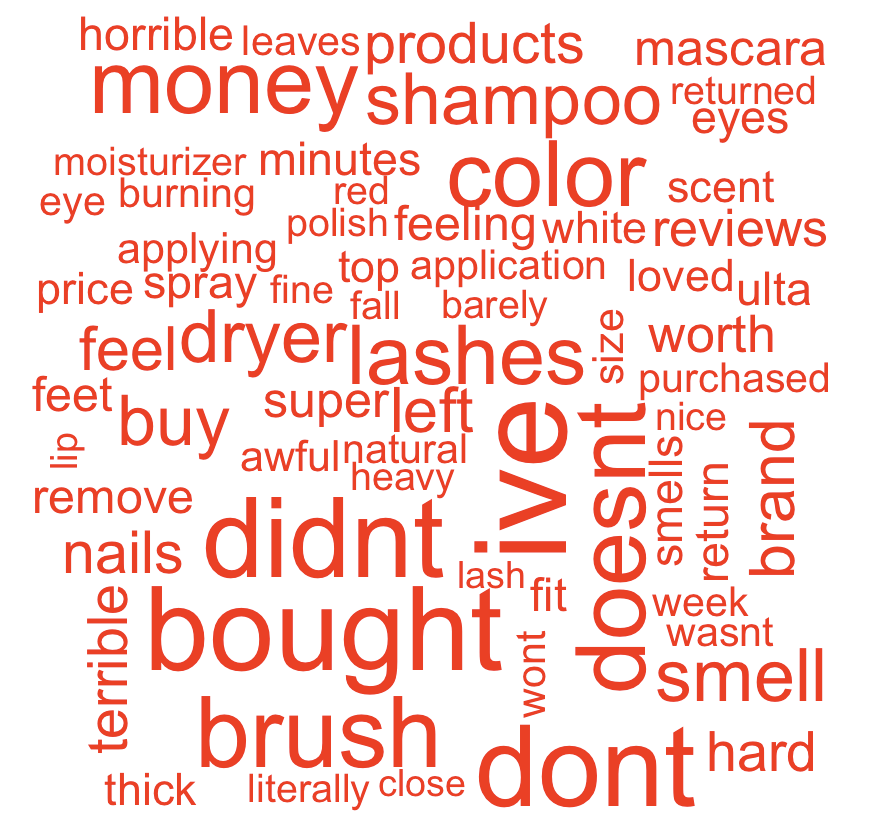
\includegraphics[height = 80mm, width=80mm]{wc_bad.png}}\hspace{1em}
    \subcaptionbox{Star-Rating $>4.5$}{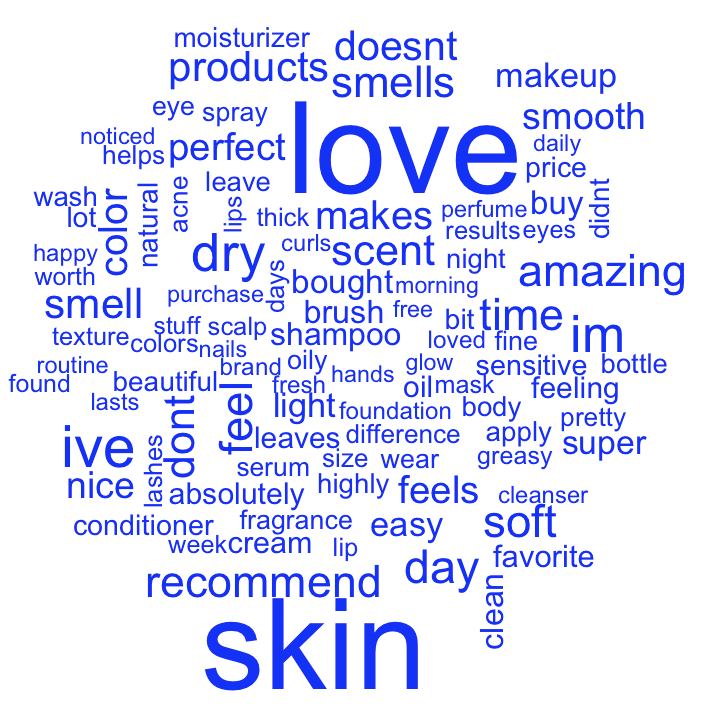
\includegraphics[height = 80mm, width=80mm]{wc_good.png}}
    \caption{Word-Clouds using 100 Most Frequently Used Terms}
    \hspace*{\fill}
\end{figure}

\

We first conducted a qualitative verification by visually comparing the normalized ratings and our predicted sentiment scores for a variety of randomly selected products. If a product had both relatively lower ratings and relatively lower sentiment scores, it would indicate that our predicted scores accurately represented true customer sentiment. Figure (2) illustrates the results for 100 randomly selected products. In general, we can see that products with lower sentiment scores generally had lower ratings, while those with higher sentiment scores had higher ratings.


\begin{figure}[ht!]
    \centering
    \hspace*{-2em}
    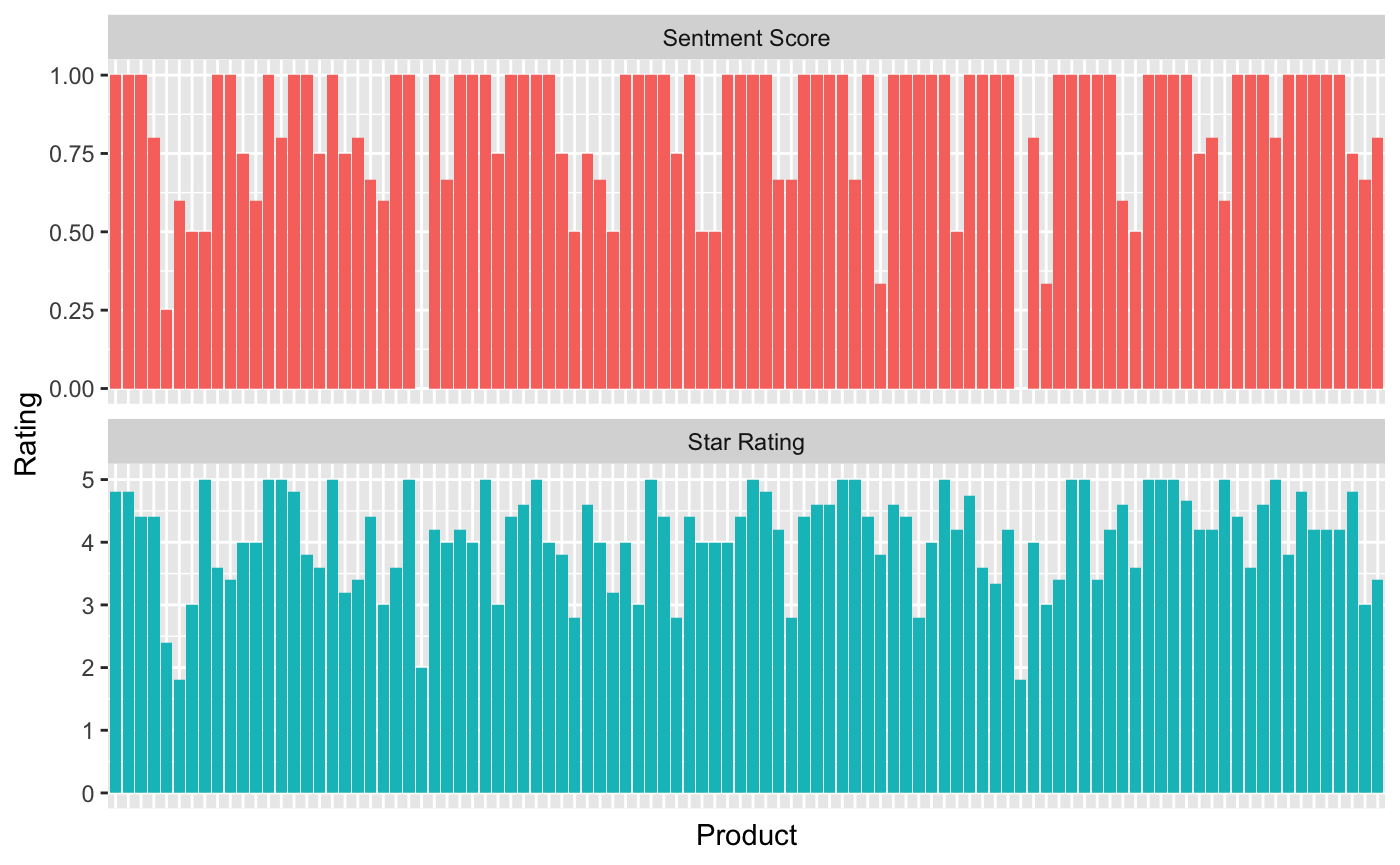
\includegraphics[height=90mm, width=150mm]{sent-vs-star.png}
    \caption{Comparing Normalized Star Rating to Predicted (Positive) Sentiment Scores}
\end{figure}

\

In addition to the visual validation, we computed the Pearson's correlation coefficient between the normalized star ratings and our predicted sentiment scores. At the $\alpha = 0.05$ level, we observed a significant positive relationship between star ratings and our predicted sentiment, with a correlation estimate of $\hat \rho = 0.44$. This suggests that as star ratings increase, our predicted sentiment scores also tend to increase. 

\

The results described above indicate that our predicted sentiment scores were able to successfully measure the true customer sentiment for a given product. However, it is important to emphasize that while we desire a positive correlation between star ratings and sentiment, our goal in predicting sentiment is not to achieve a perfect match with the ratings. Rather, we aim for our predicted sentiments to provide brands with more insightful characterizations of each customer's review than ratings alone.



\subsection{Revealing Word Trends with Term Frequencies \& TF-IDF}

We now move on to assess the word frequencies within the product descriptions based on the rating of the individual products and the overall sentiment found in the previous section. Figure (3) displays the most common words in product descriptions for products with a positive sentiment (right), and the most common words in product descriptions for products with a negative sentiment (left). We also generated a similar plot using the original rating instead of our predicted sentiments. Unfortunately, both sets of plots do not tell us anything insightful. We can see the plots have too much overlap of frequently used words because certain words (e.g. skin, hair, oil) dominate many product descriptions. 

\begin{figure}[ht!]
    \centering
    \hspace*{-3em}
    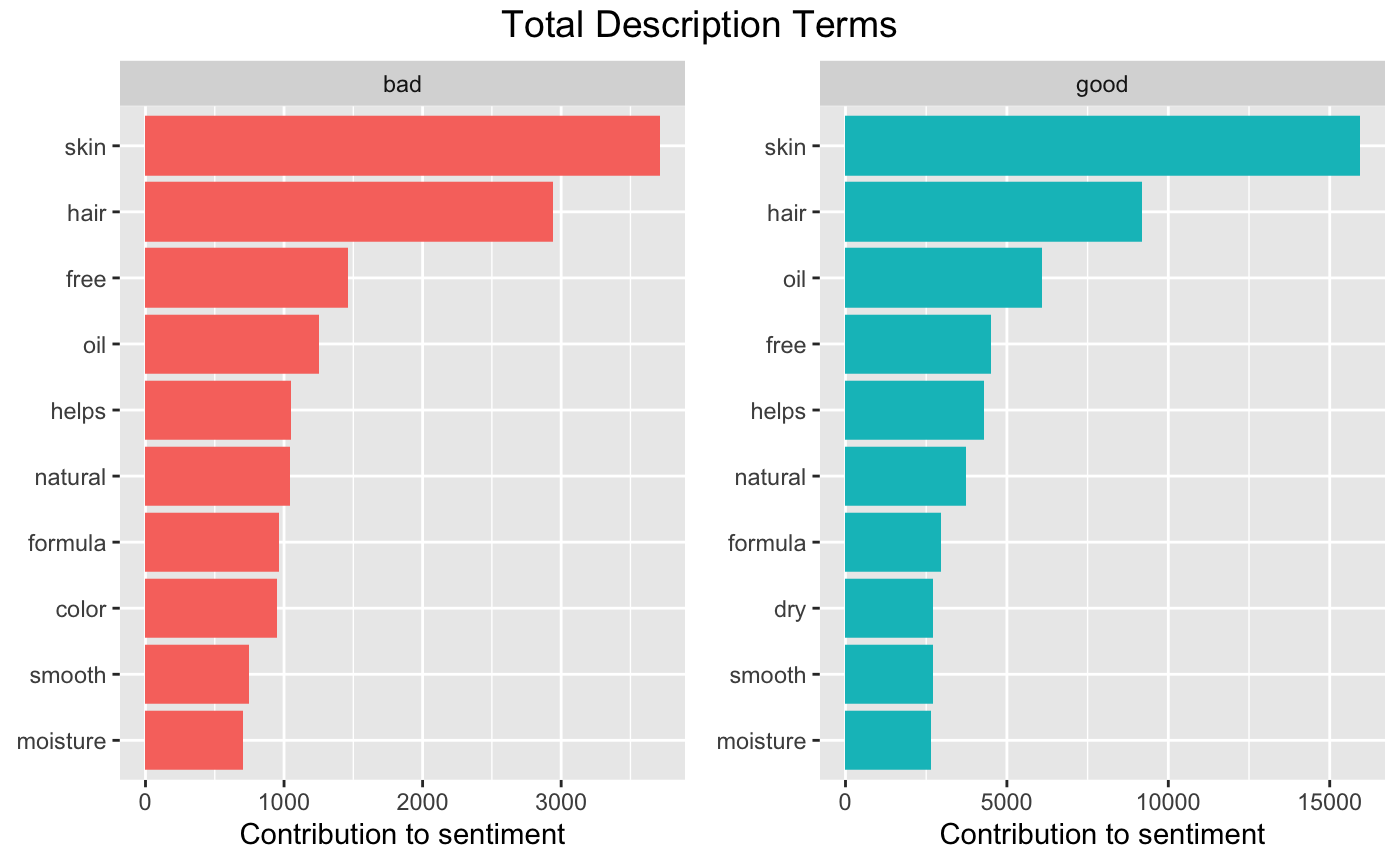
\includegraphics[height=90mm, width=150mm]{freq_total.png}
    \caption{Most Frequent Words Used in Descriptions (Grouped by Predicted Sentiment)}
\end{figure}

\

One solution to this problem may be to assess the \textit{Term-Frequency Inverse-Document-Frequency} (tf-tdf) values instead of pure term frequencies to reduce the presence of overlapping terms between the positive and negative sentiment groups. However, we are also interested in seeing exactly how much more a word is associated with a given sentiment group. Therefore, we decided to find the terms associated with the largest absolute difference in relative frequencies. Figure (4) displays the words with the largest positive and negative differences between the normalized frequencies for the two sentiment groups. We can see that words related to hair care or eye makeup, such as hair, scalp, lashes, and mascara, appear to be associated with negative customer sentiment. On the other hand, we can see that words related to cleansers and lip \& cheek makeups, such as oil, wash, skins, blush, and lip, appear to be associated with positive customer sentiment. 

\begin{figure}[ht!]
    \centering
    \hspace*{-3em}
    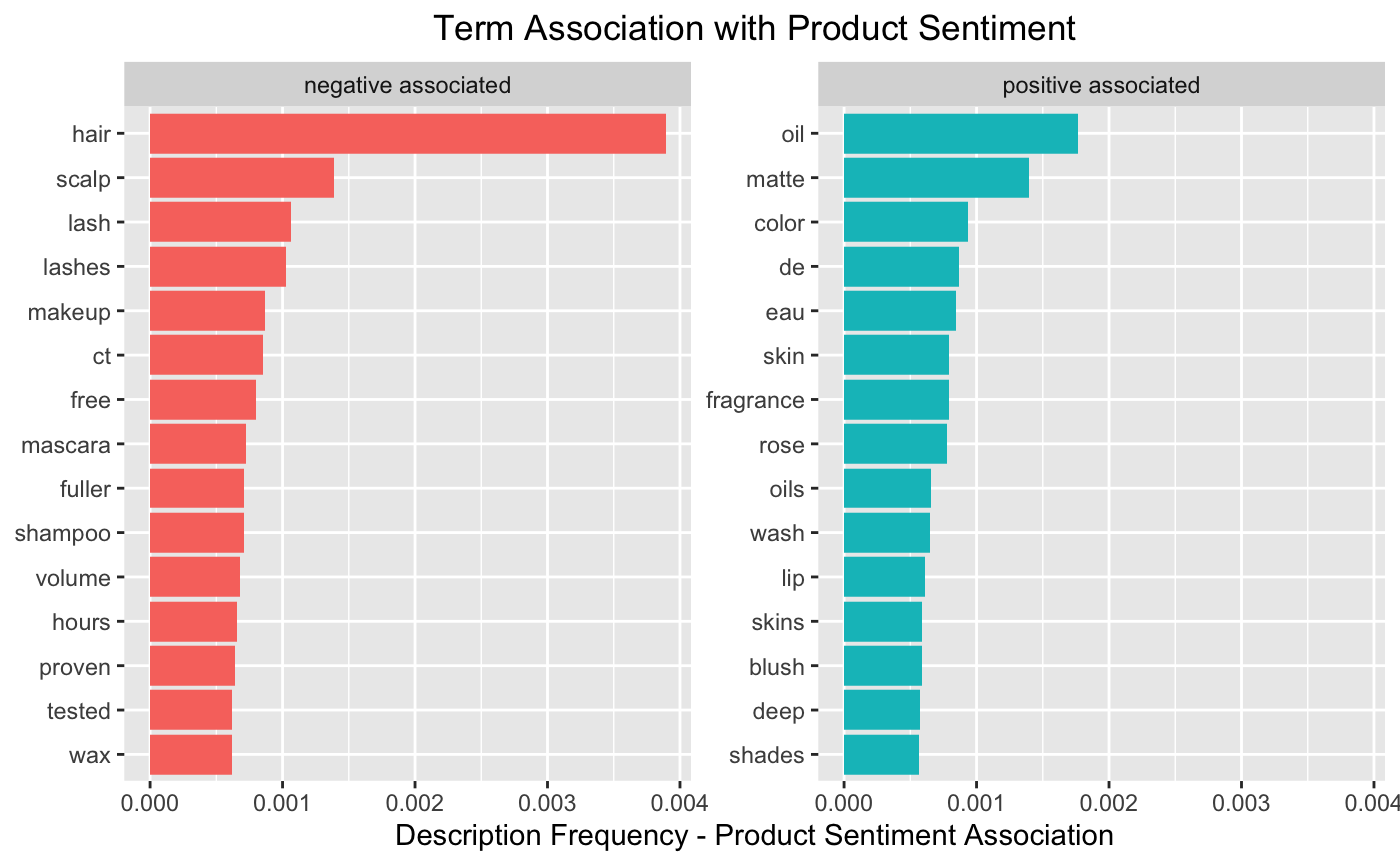
\includegraphics[height=90mm, width=150mm]{word_assocs_total.png}
    \caption{Words with Largest Differences in Normalized Frequency}
\end{figure}

\

Our term-associations analysis continues by examining words with the highest tf-idf scores for brands or product categories with the best and worst overall customer sentiment and rating. To determine the overall sentiment scores for entire brands or product categories, we merged the predicted sentiment scores from Section 3.1 with the normalized ratings to create a ``combined rating'' measure, denoted as the weighted average of sentiment and rating. 

\

The optimal weighting for the combined rating was determined through tuning, with a value of $\omega = 0.6$ assigned to the sentiment score and $1-\omega$ assigned to the rating. By assigning greater weight to sentiment scores, we aimed to extract more meaningful insights from the review text than from star ratings alone. Among the brands analyzed, Rituals, Montblanc, and Azzaro achieved the highest mixed ratings, while Nair, Nads Natural, and Hollywood Fashion Secrets received the lowest combined ratings. Figures (5) and (6) present these six brands along with their largest corresponding tf-idf scores. 

\begin{figure}[ht!]
    \centering
    \hspace*{-3em}
    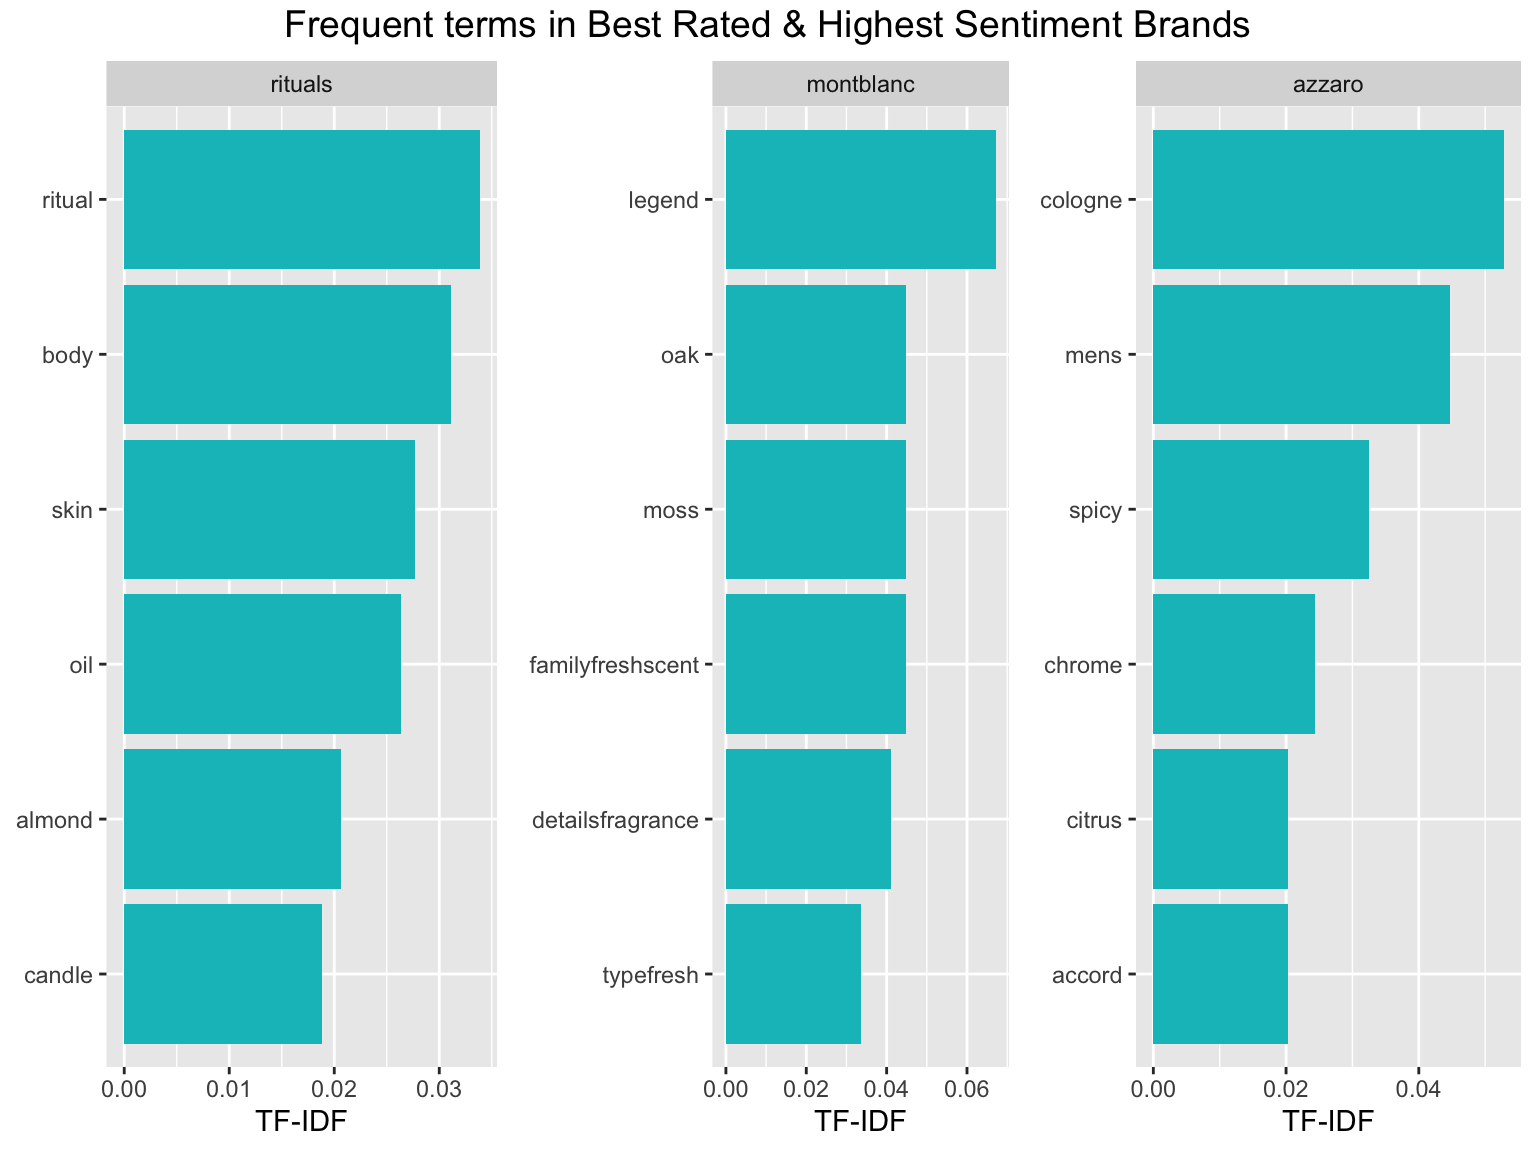
\includegraphics[height=90mm, width=130mm]{best_mr_brands.png}
    \caption{Highest Combined Rated Brands}
\end{figure}

\begin{figure}[ht!]
    \centering
    \hspace*{-3em}
    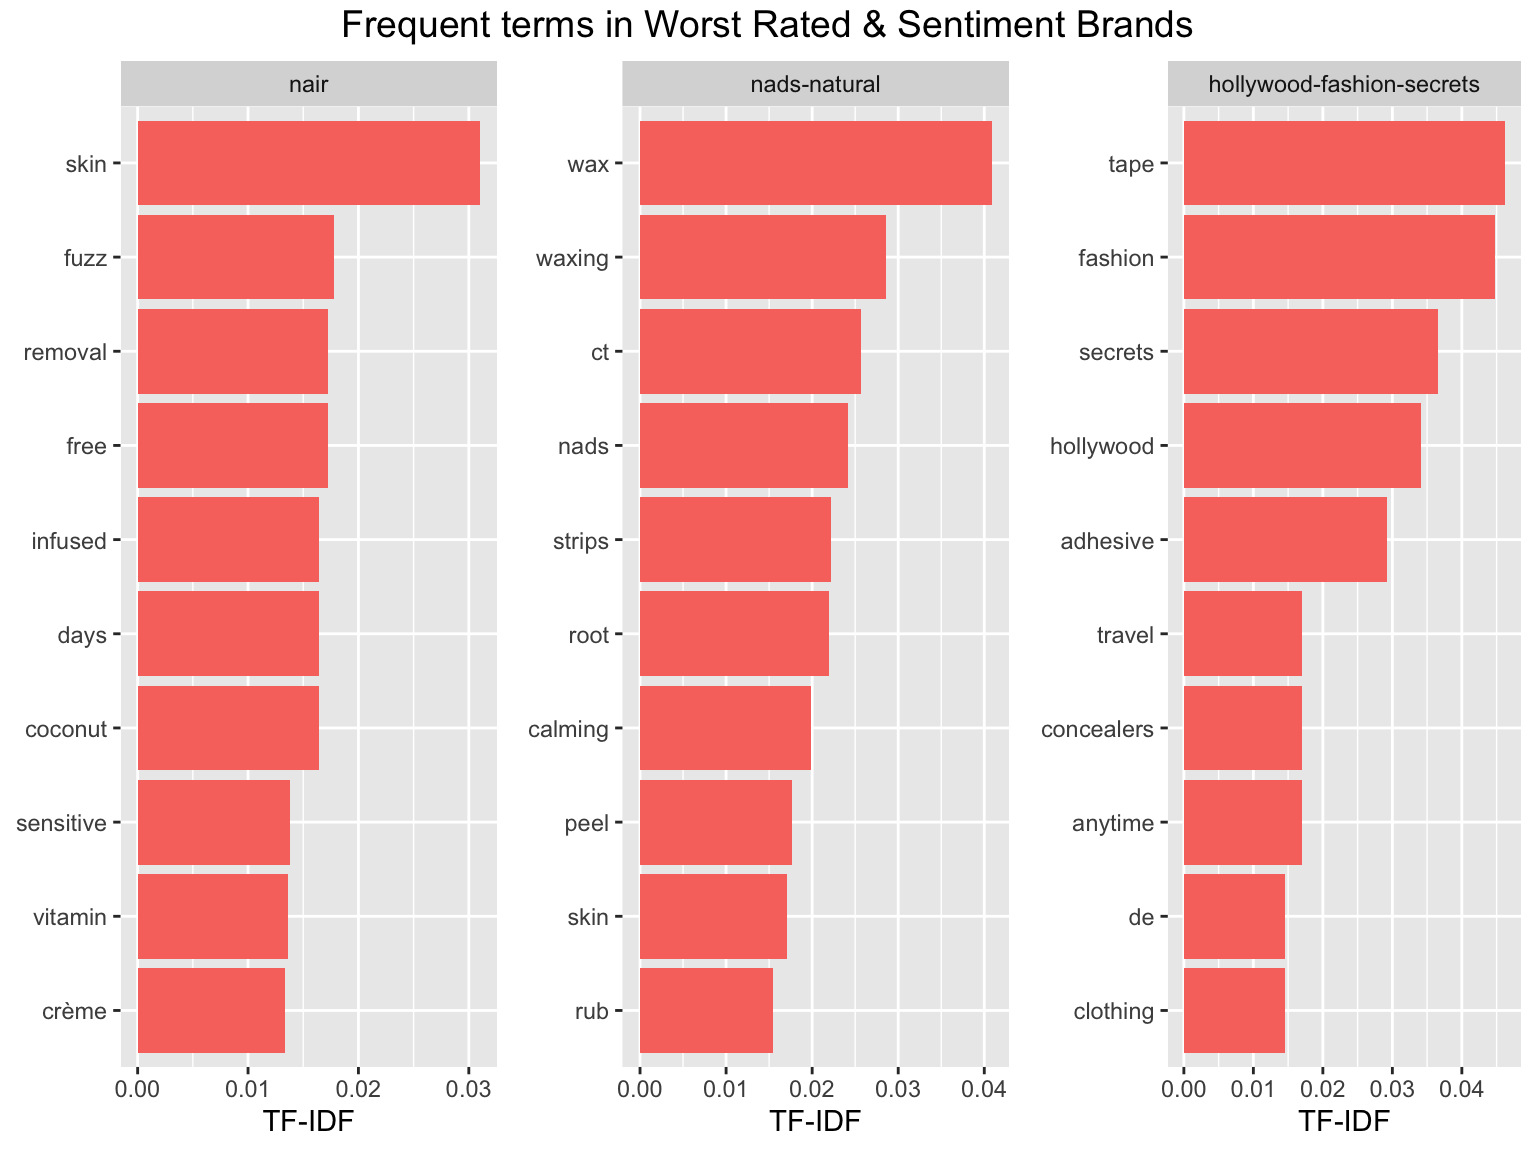
\includegraphics[height=90mm, width=130mm]{worst_mr_brands.png}
    \caption{Lowest Combined Rated Brands}
\end{figure}

\

Figure (5) reveals that two out of the three brands with the highest combined sentiment and rating scores primarily focus on cologne and fragrance (Montblanc and Azzaro). Intriguingly, Figure (6) demonstrates that the brands associated with the lowest combined sentiment and rating scores are primarily linked to hair removal, waxing, or body taping. 

\

Continuing our analysis, we extended our investigation to product categories using the combined ratings as the primary metric. Similar to the brand analysis, we explored the categories that obtained the highest and lowest combined ratings. Notably, categories such as beard care, cologne, and body lotions achieved the highest combined ratings, aligning with our findings from the previously identified ``best'' brands. Conversely, categories such as hair rollers, eye makeup removal, and hair removal tools received the lowest mixed ratings, which remained fairly consistent with the ``worst'' brands found earlier. We should also note that we only used brands with more than 25 reviews and product categories with more than 30 reviews to prevent large variances from small pools of reviews affecting the accuracy of our analysis.

\

In addition to our previous analysis, we acknowledge the importance for brands to address the following inquiries:

\begin{enumerate}
    \item Which product categories exhibit the highest customer sentiment and ratings for our brand?
    \item Which other brands receive the best customer sentiment and ratings within a specific product category?
\end{enumerate}

To address the first question, we illustrate our approach using two prominent brands: Peach \& Lily and Colourpop. For each brand, we grouped their products by available categories and identified the categories with the highest and lowest combined ratings. We prioritized the combined rating to extract comprehensive insights from both customer reviews and star ratings. It is plausible that the predicted sentiment scores derived from customer reviews offer more valuable information than the star ratings alone. Table (1) showcases the product categories associated with the highest and lowest combined ratings for each brand. The findings indicate that Peach \& Lily customers display a preference for Face Peels \& Exfoliators, while expressing less enthusiasm for Cleansing Balms \& Oils. Similarly, customers exhibit favorable sentiment towards Colourpop's Lip Linear, while showing less satisfaction with Colourpop's Mascara, as evident from their reviews and ratings.

\begin{table}[h!]
    \centering
    \begin{tabular}{| c | c | c |} 
    \hline
    \textbf{Brand} & \textbf{Best Product Category} & \textbf{Worst Product Category} \\ 
    \hline
    \hline
    Peach \& Lily  & Face Peels \& Exfoliators & Cleansing Balms \& Oils \\
    \hline
    Colourpop  & Lip Liner & Mascara \\
    \hline  
    \end{tabular}
    \caption{Best and Worst Product Categories Associated with Each Brand}
\end{table}

\

To address the second question, we illustrate our methodology using three significant product categories: ``Shampoo'', ``Face Moisturizer'', and ``Mascara''. Similar to our approach in answering the first question, we leverage the combined scores of customer ratings and predicted customer sentiments to identify the brands with the highest and lowest rankings within each category. The outcomes of this analysis are presented in Table (2). Notably, we observe that Morphe Cosmetics, a well-known brand, exhibits the lowest combined rating among its available mascara products, which offers an interesting insight.

\begin{table}[h!]
    \centering
    \begin{tabular}{| c | c | c |} 
    \hline
    \textbf{Product Category} & \textbf{Best Brand} & \textbf{Worst Brand} \\ 
    \hline
    \hline
    Shampoo & Blind Barber & Its A 10 \\
    \hline
    Face Moisturizer & Black Opal Beauty & BYOMA \\
    \hline  
    Mascara & Elf Cosmetics & Morphe Cosmetics \\
    \hline  
    \end{tabular}
    \caption{Best and Worst Brands Associated with Each Category}
\end{table}

\subsection{Discovering Commonalities With Topic Modeling}

In this section, we utilize \textit{Latent Dirichlet Allocation} (LDA) to build topic models on our text data. Each topic in the model represents a mixture of words, and our objective is to identify the optimal combination of words associated with each topic. To achieve this, we treat the set of product descriptions for each brand as a separate ``document'' to determine the most suitable mixture of topics that characterizes each brand. After fitting multiple LDA models, we determined that a choice of $k=3$ topics provides the most effective separation of themes. By employing these generated topics, we can identify commonalities among the brands and group them based on shared topics, thereby gaining insights into brands' similarities derived from their product descriptions.

\begin{figure}[ht!]
    \centering
    \hspace*{-4em}
    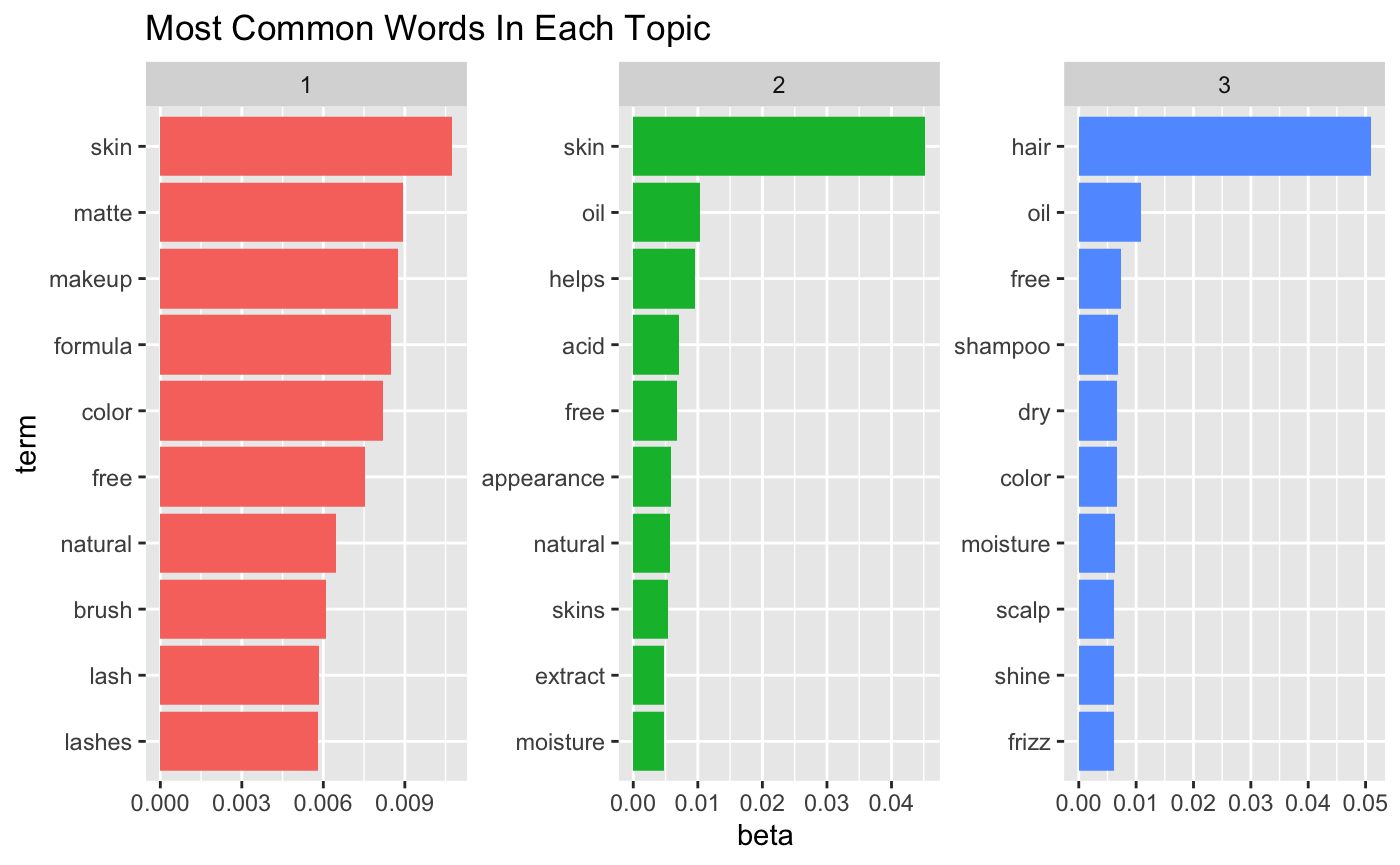
\includegraphics[height=80mm, width=130mm]{topics.png}
    \caption{Most Common Terms Within Each Topic (Using $\beta$ Probabilities)}
\end{figure}

\

We extract the per-topic-per-word probabilities ($\beta$) from our model, which enables us to identify the 10 most frequently occurring terms within each topic (Figure (7)). Through visual examination of Figure (7), we can clearly discern the characteristics of each topic based on its most common terms, considering the context of our dataset. For instance, Topic \#1 appears to pertain to general makeup or lashes, Topic \#2 is associated with facial and body cleansers or moisturizers, and Topic \#3 predominantly relates to hair care.

\

Next, we analyze each brand's probability of being associated with each topic. By extracting the per-document-per-topic probabilities ($\gamma$) from our model, we estimate the proportion of words from each brand that originate from a specific topic. Using these probabilities, we identify the top 10 brands that are most strongly associated with each topic (i.e., those with the highest $\gamma$ values) and present them in Table (3). 


\begin{table}[h!]
    \centering
    \begin{tabular}{| c | c | c | c |} 
    \hline
    \textbf{Ranking} & \textbf{Topic \#1} & \textbf{Topic \#2} &  \textbf{Topic \#3}\\ 
    \hline
    \hline
     1  & NYX Professional Makeup & Dermalogica & Joico \\
     \hline  
     2  & Anastasia Beverly Hills & Neutrogena & Living Proof \\
     \hline  
     3  & Dashing Diva & La Roche Posay & Redken \\
     \hline  
     4  & Kiss & Cerave & Paul Mitchell \\
     \hline  
     5  & Real Techniques &	Peter Thomas Roth &	Drybar \\
     \hline  
     6  & Maybelline & Fresh & Bumble-Bumble \\ 
     \hline  
     7  & Ardell & Hempz & Devacurl \\
     \hline  
     8  & Fenty Beauty by Rihanna & Vichy & Lanza \\
     \hline  
     9  & Makeup Revolution & Murad & Fekkai \\
     \hline  
     10 & Juvias Place & Boscia & Not Your Mothers \\
    \hline  
    \end{tabular}
    \caption{Top 10 Brands Most Associated with Topics}
\end{table}

Consistent with our topic characterization, Table 3 reveals that makeup brands like NYX and Anastasia Beverly Hills exhibit a strong association with Topic \#1, skincare companies such as Dermalogica and Neutrogena are highly associated with Topic \#2, and hair care brands like Joico and Living Proof demonstrate a strong association with Topic \#3.


\subsection{Contrasting Term Frequencies in Topics \& Makeup Brands}

For our final exploratory analysis, we proceed to compare and contrast the term frequency proportions among the $k=3$ generated topics from the previous section. Scatter plots were utilized to visually depict the correlation between topics and evaluate the words responsible for their associations. Pearson's correlation coefficients were then employed to quantify the level of correlation in term frequencies between topics. Figure (8) presents the correlation plots between Topic \#1 and Topics \#2 \& \#3.

\begin{figure}[ht!]
    \centering
    \hspace*{-4em}
    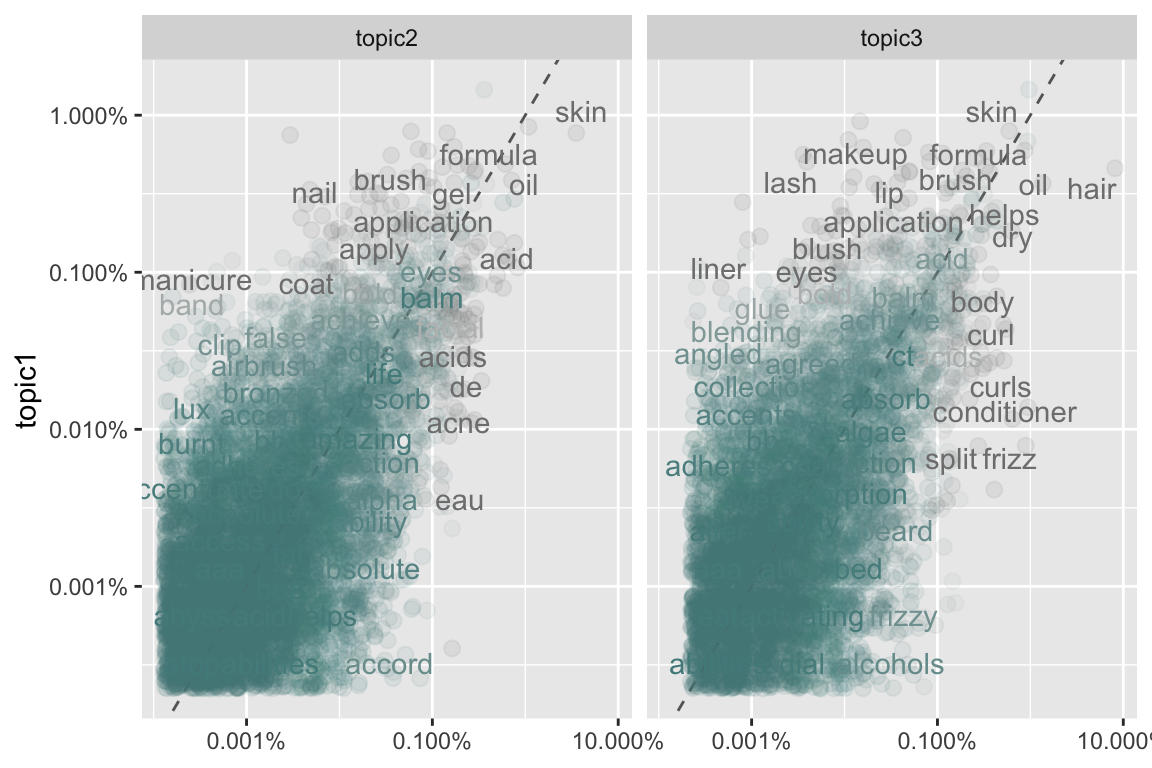
\includegraphics[height=65mm, width=120mm]{corrplot1.png}
    \caption{Scatter Plots for Word Frequencies between Topics}
\end{figure}

\

In these plots, words that lie closer to the line exhibit similar frequencies in both topics, while words that deviate further from the line are more prominent in one topic compared to the other. For example, Figure (8) illustrates that words such as ``skin'' and ``formula'' demonstrate similar frequencies (at the upper frequency end) in both Topic \#1 and Topic \#2. Conversely, words like ``nail'' or ``coat'' are more prevalent in Topic \#1 than in Topic \#2.

\

Taking a closer look at Figure (8), we observe that the words in the Topic \#1 - Topic \#2 panel exhibit a closer alignment with the zero-slope line compared to the Topic \#1 - Topic \#3 panel. Specifically, the estimated correlation coefficient between Topic \#1 and Topic \#2 is 0.64, while the estimated correlation coefficient between Topic \#1 and Topic \#3 is only 0.40. Considering that Topic \#1 represents makeup brands, Topic \#2 represents skin care brands, and Topic \#3 represents hair care brands, this finding indicates that word frequencies between makeup brands and skin care brands are more closely related than word frequencies between makeup brands and hair care brands. This can be attributed to the fact that makeup and skin care products are often applied to similar areas, leading to a significant overlap in the terms used in their product descriptions.

\

Furthermore, we conduct a similar correlation analysis based on the word frequencies from three prominent makeup brands: L'Oreal, Colourpop, and Maybelline. Again, the objective is to assess the similarities and differences among these brands based on the language used in their product descriptions. The correlation plots between L'Oreal and Colourpop, as well as L'Oreal and Maybelline, are presented in Figure (9).

\begin{figure}[ht!]
    \centering
    \hspace*{-4em}
    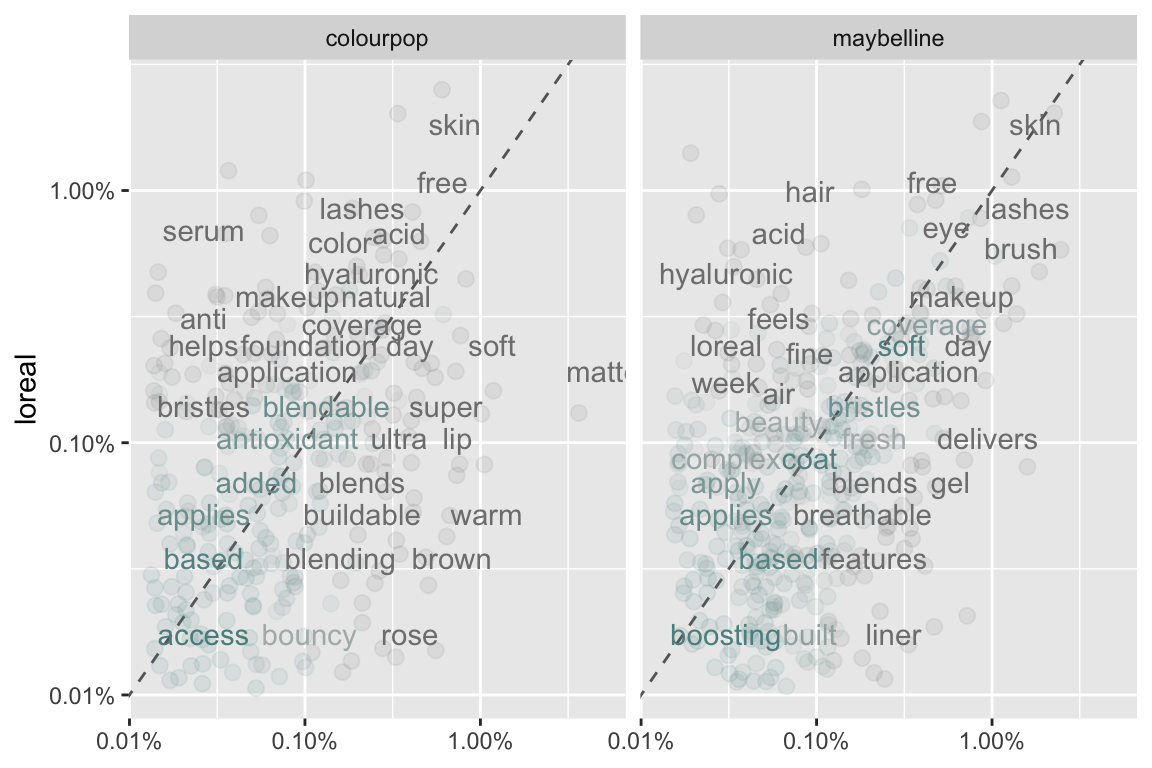
\includegraphics[height=65mm, width=120mm]{corrplot2.png}
    \caption{Scatter Plots for Word Frequencies between Topics}
\end{figure}

\

Upon examination, we immediately observe that the words in the L'Oreal - Maybelline panel appear much closer to the zero-slope line compared to the L'Oreal - Colourpop panel. Although all three brands exclusively focus on makeup, Colourpop stands out with their choice of descriptive words for their product descriptions. Notably, terms such as ``blending'', ``brown'', ``warm'', ``matte'', and ``bouncy'' exhibit significantly higher relative frequencies in Colourpop products compared to L'Oreal (and Maybelline). As anticipated from the scatter plots, the estimated correlation between L'Oreal and Maybelline is remarkably high at 0.65, whereas the estimated correlation between L'Oreal and Colourpop is substantially lower at 0.16.

\

So, what distinguishes Colourpop from L'Oreal (and Maybelline)? To delve into this disparity, we utilize the log odds ratio:

$$\text{Log Odds Ratio} = \ln \left( \frac{\left[ \frac{n+1}{\text{total}+1} \right]_{\text{L'Oreal}}}{\left[ \frac{n+1}{\text{total}+1} \right]_{\text{Colourpop}}} \right)$$

to identify the top 15 most distinctive words for both L'Oreal and Colourpop. These distinctive terms are then visualized in Figure (10) to shed light on the factors contributing to the dissimilarity between these brands. Notably, L'Oreal's distinctive words, such as ``wrinkles'', ``aging'','' and ``retinol'', are associated with slightly older customers seeking anti-aging products. In contrast, Colourpop's distinct terms consist of more youthful and vibrant descriptors, including ``peach'', ``chocolate'', ``pink'', ``icy'', ``glitter'', ``silver'', ``gold'', and ``metallic''. It is worth mentioning that L'Oreal (and Maybelline) has a long-standing history dating back to the early 1900s, whereas Colourpop was founded in 2014. Hence, based on the word frequencies in the product descriptions, it appears that Colourpop's target customers are generally younger, possibly belonging to the Gen-Z demographic, while L'Oreal tends to cater to a slightly older customer base.

\begin{figure}[ht!]
    \centering
    \hspace*{-4em}
    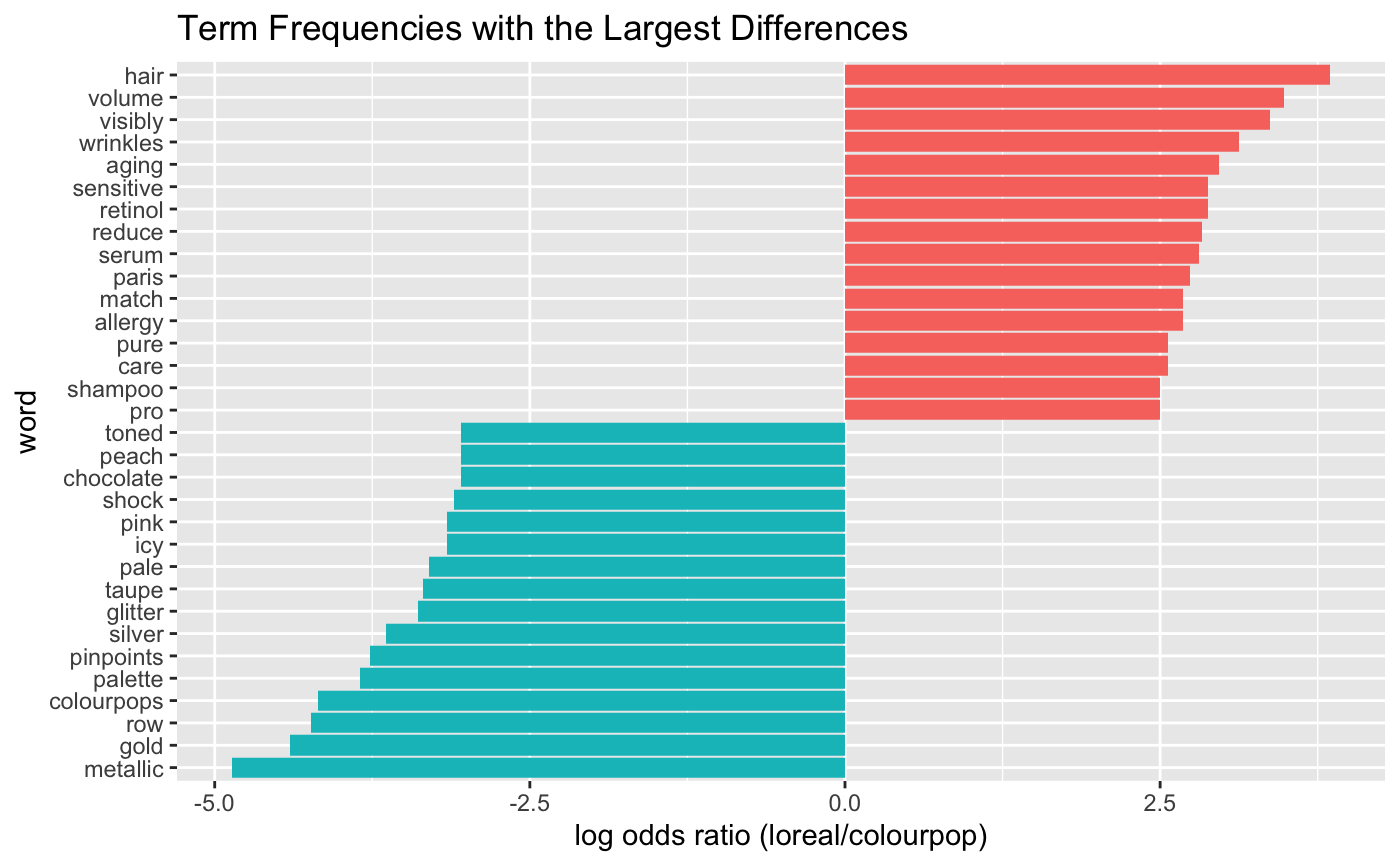
\includegraphics[height=100mm, width=130mm]{lorealVScp.png}
    \caption{Most Distinctive Words for L'Oreal and Colourpop}
\end{figure}

\section{Modeling}

Following the exploratory analyses, we proceed to model the specific relationships within our collected data. Our approach involves training, tuning, and testing each model. However, we also intend to capitalize on the unique characteristics or attributes of each model to gain insights and interpret their significance within the given context.

\subsection{Predicting Average Star Ratings From Reviews}

The initial model we develop focuses on predicting the average star rating of a product based on customer reviews. This aims to assess how well the text in the reviews can estimate the overall product rating.

\

Before proceeding with model training, it is important to mention that we performed additional preprocessing steps, including stemming and removal of sparse terms with a maximum allowed sparsity level of $\texttt{sparse}=0.995$. By removing very sparse terms, we significantly reduced the feature space without compromising the predictive performance of our model. Stemming was also applied to reduce the number of words inputted to the model and to minimize confusion among words with similar meanings.

\

Next, we trained a random forest (regressor) model using 80\% of the text data from the product reviews, along with their corresponding ratings. A grid search with 4-fold cross-validation was employed to tune the hyperparameters of the random forest model. The \textit{root-mean-squared error} (RMSE) served as our tuning metric, and we utilized visual aids, such as the plot in Figure (11), to determine the optimal hyperparameters. For example, Figure (11) helped us identify that the ideal number of terms to randomly sample at each split is 234.

\begin{figure}[ht!]
    \centering
    \hspace*{-2em}
    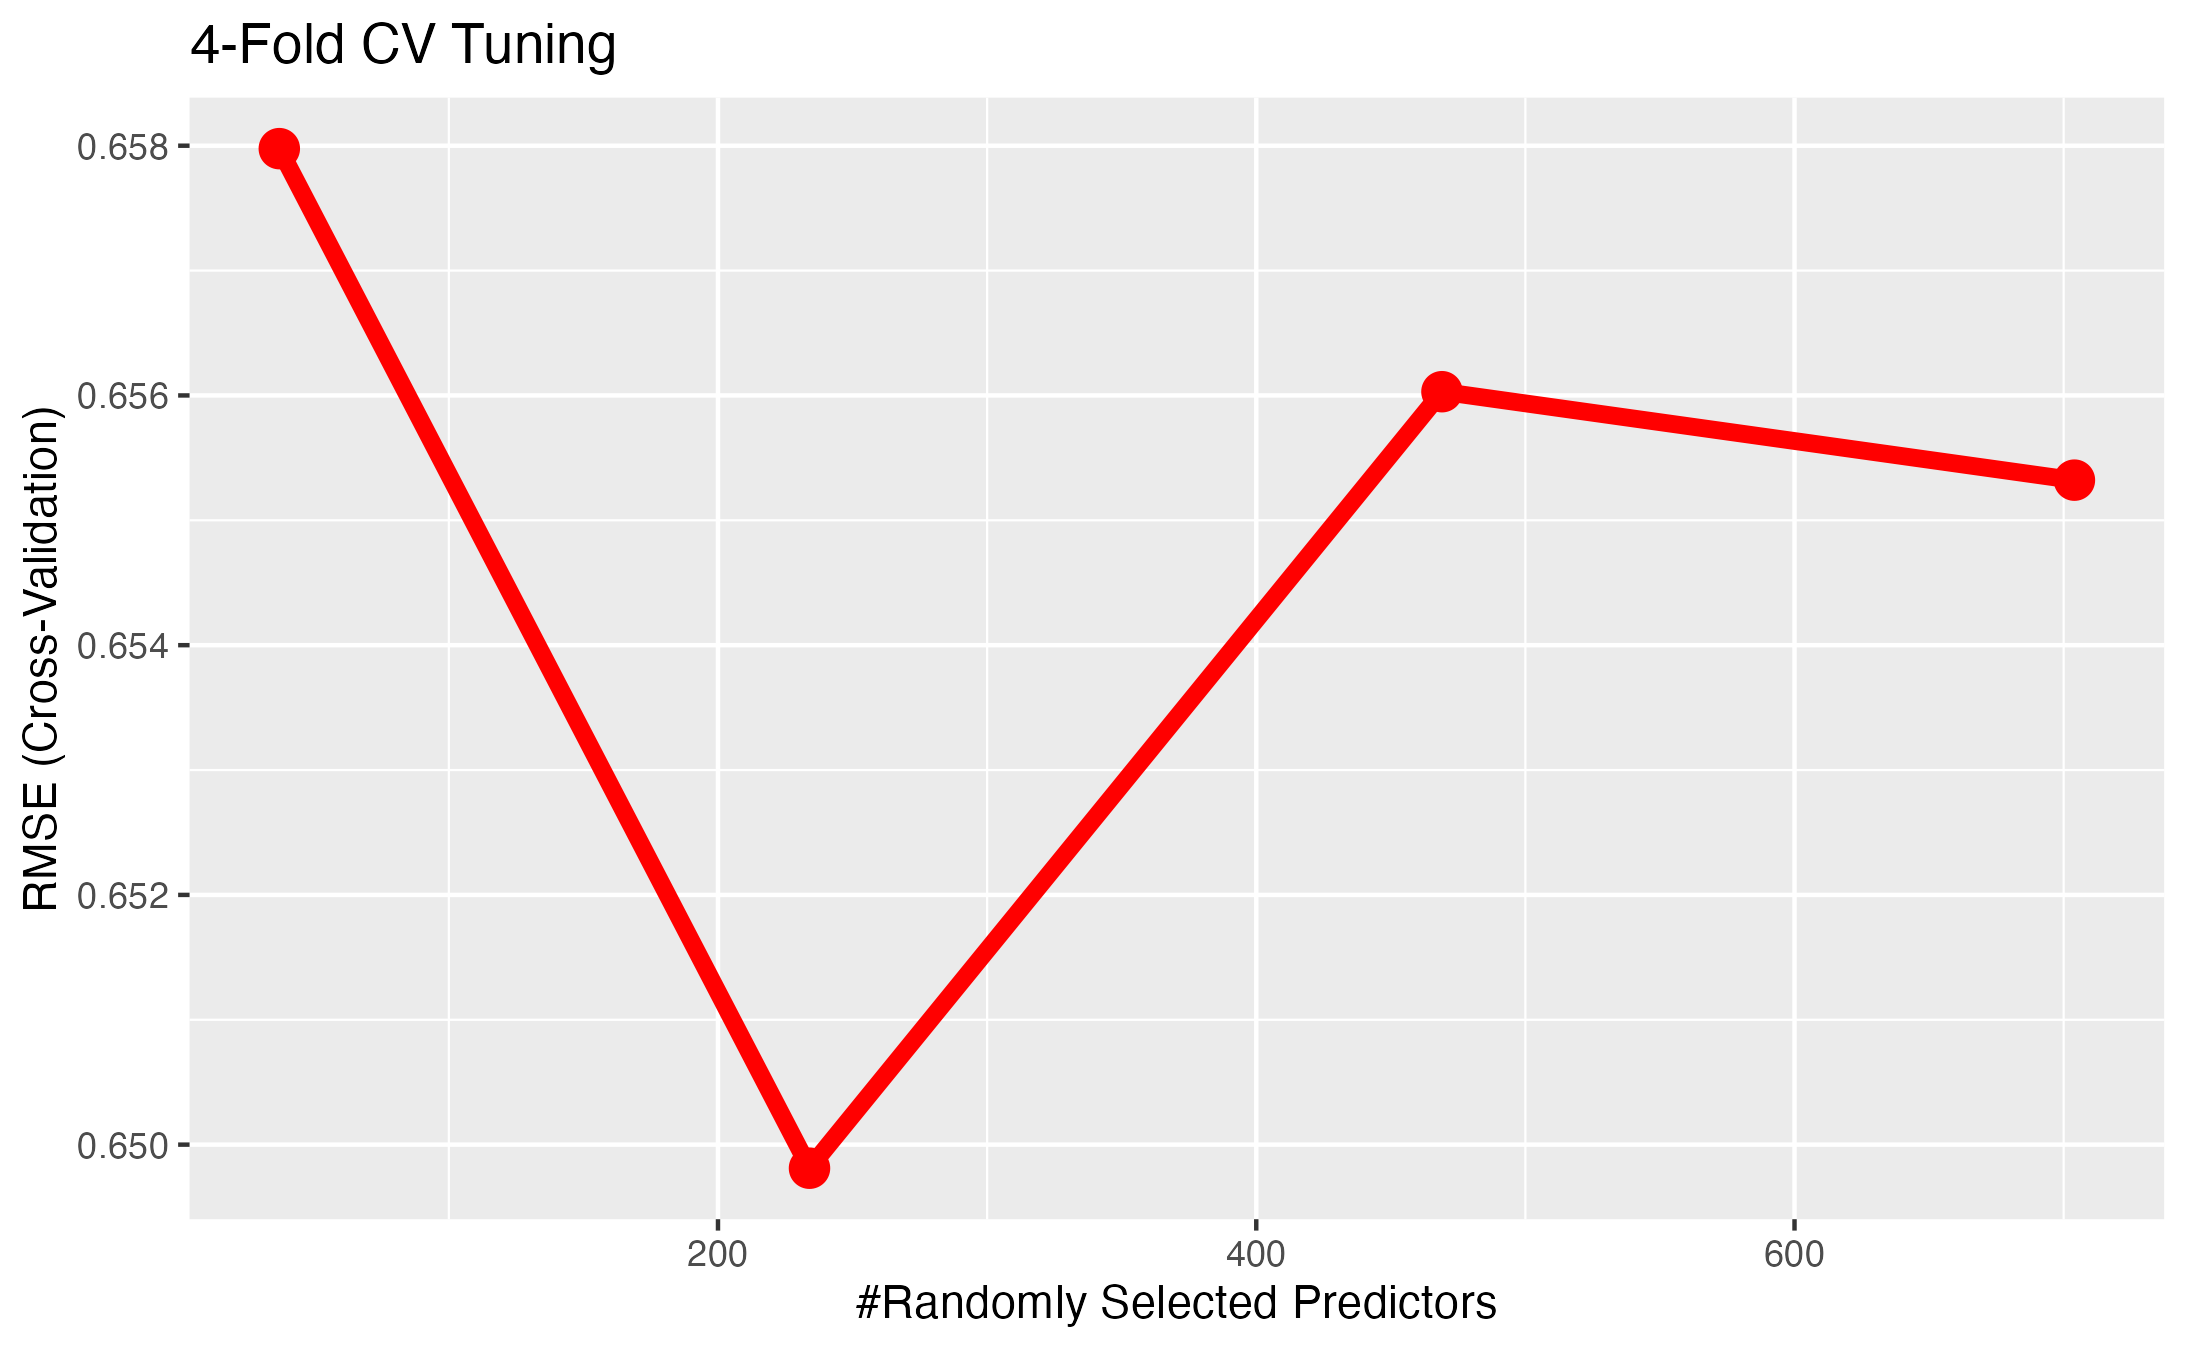
\includegraphics[height=85mm, width=105mm]{rev_cv_rf_tuning.png}
    \caption{Grid Search Tuning Plot for \texttt{mtry} Hyperparameter}
\end{figure}

\

Once the parameters were tuned, we re-trained the random forest model using the entire 80\% training data, utilizing a total of $\texttt{n}=500$ trees and $\texttt{mtry}=234$ terms randomly sampled at each split. Due to the increased number of trees and the large number of predictors (words), the training process for the final model took approximately 18 minutes. The reported training RMSE was 0.2675, indicating that, on average, our model predicted within approximately 0.2675 stars for the products in our 80\% training data.

\

We proceeded with formal testing of our tuned random forest regressor on a separate test set comprising the remaining 20\% of unseen text data. We found that our model achieved an RMSE of 0.6176 on the test data, indicating that our model was able to predict within about 0.6176 stars (on average) for the unseen products. For additional context, we should note that each product's average star-rating could be between 0 and 5 stars. In fact, we found that our random-forest regressor achieved an R-Squared of 0.4270 on the test data, which implies that it was able to explain a significant proportion of the variance in the star ratings. Therefore, we concluded that our tuned random-forest regressor was able to successfully generalize to unseen products and demonstrated excellent predictive performance.

\

Given the strong predictive capabilities of our model, we generated a feature importance plot, displayed in Figure (12). The x-axis represents a measure of the total increase in node purity that results from splits over that variable, averaged over all 500 trees. In the case of our random forest regressor, the variable importance is assessed by considering how much the model error (RSS) increases when a particular variable is randomly permuted or shuffled (denoted by \texttt{IncNodePurity}). For improved interpretability, we color-coded the terms in Figure (12) based on their sentiment using the \textit{Bing Sentiment Lexicon}. Interestingly, among the top 15 most important words for star-rating predictions, we can see that only 2 had a positive sentiment.

\begin{figure}[ht!]
    \centering
    \hspace*{-2em}
    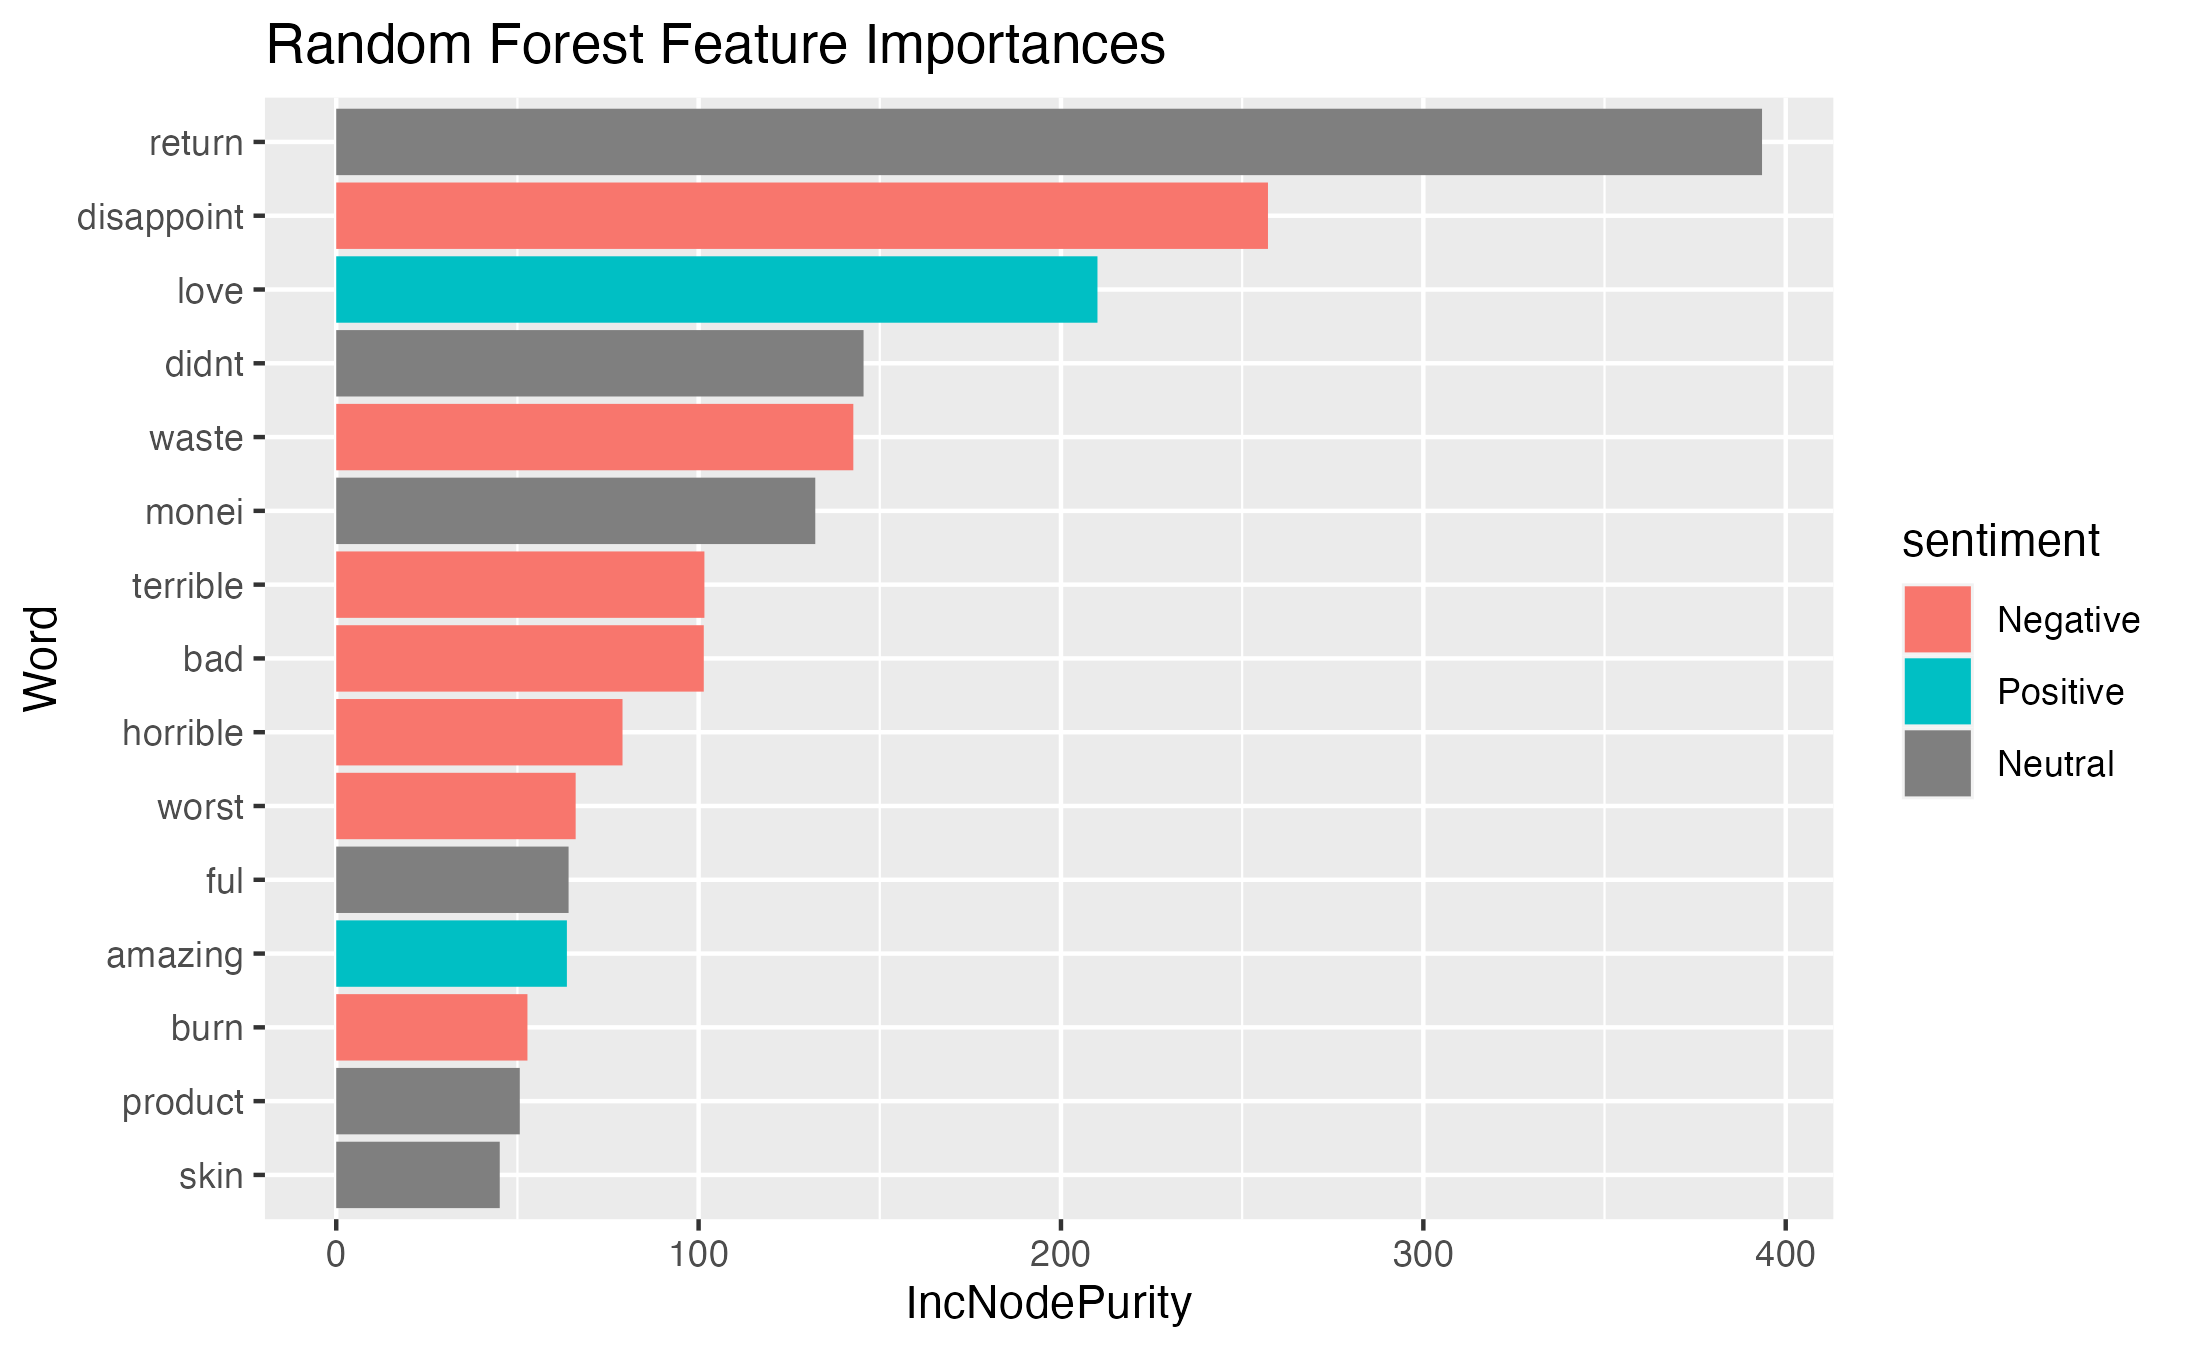
\includegraphics[height=80mm, width=105mm]{reviews_feat_imp.png}
    \caption{Feature Importance for the Tuned Random Forest Regressor}
\end{figure}


\

We observe that terms such as ``return'', ``disappoint'', and ``love'' have the greatest impact on our model's predictions. This aligns with intuition, as these words clearly reflect satisfaction levels associated with a product. For instance, we would expect products with reviews containing sentences such as ``I am \textit{disappointed}'' or ``I \textit{returned} this product'' to typically receive lower ratings, while products with reviews containing a sentence like ``I \textit{loved} this product'' to generally receive higher ratings. The remaining words displayed in Figure (12), along with their associated sentiment, offer additional context regarding which words from the reviews had the most significant influence on predicting product ratings.


\subsection{Unveiling the Price-Sentiment Nexus}

In this section, we aim to explore the relationship between product price and customer sentiment, challenging the assumption that higher prices always indicate a more negative sentiment. To investigate this, we employ the binomial logistic regression model with product price as the predictor variable and sentiment (positive or negative) as the response variable. The binary response variable is derived from the predicted sentiment obtained in our earlier analysis (Section 3.1). Specifically, a positive response corresponds to a product with a predicted sentiment score greater than 0.5, while a negative response corresponds to a product with a predicted sentiment score less than 0.5. Products with a predicted sentiment score of exactly 0.5 were excluded from consideration.

\

To begin, we examined the overall relationship between product price and customer sentiment by fitting a single logistic regression model that incorporates \textit{all} products from every brand and product category. Table (4) presents a summary of this globally fitted model. The results in Table (4) demonstrate that price is a significant predictor of sentiment at the $\alpha=0.05$ level. Since the estimated coefficient $\hat{\beta}{\texttt{price}}>0$, we conclude that, across all product classes, an increase in price corresponds to a more positive sentiment. Specifically, on average, a \$10 increase in product price leads to a 5.6\% increase in the odds of the product receiving a positive sentiment (calculated as $e^{10\hat{\beta}{\texttt{price}}} = 1.056$).


\begin{table}[h!]
    \centering
    \begin{tabular}{| c | c | c | c | c |} 
    \hline
    \textbf{Variable} &  \textbf{Estimate} &  \textbf{Std. Error} &  \textbf{$Z$ value} &  \textbf{Pr($>|Z|$)} \\ 
    \hline
    \hline
    \texttt{Intercept} & 2.474844 & 0.053189 & 46.529  & $\approx 0$\\
    \hline
    \texttt{price} & 0.005441 &  0.001489 & 3.654 & $\approx 0.0003$ \\
    \hline  
    \end{tabular}
    \caption{Summary of Global Logistic Regression Model}
\end{table}

It is important to note that the results obtained from our initial logistic regression model provide insights into the global relationship between product price and customer sentiment. However, to examine this relationship on a more granular level for individual brands and product categories, we need to train logistic regression models using products specific to each brand or product category. As a result, we fitted numerous logistic regression models to evaluate how the association between price and sentiment varies across different product types and brands.

\

We began by focusing our investigation on products within each individual brand. Over 600 logistic regression models were fit to analyze the relationship between product price and sentiment within each brand. Subsequently, we filtered out any models (brands) that exhibited an insignificant relationship between price and sentiment, which could be due to either a limited number of products offered by the brand or a genuinely insignificant relationship. Table (5) presents the seven remaining brands that demonstrated a significant association between product price and sentiment at the $\alpha = 0.05$ level.

\begin{table}[h!]
    \centering
    \begin{tabular}{| c | c | c | c | c | c |} 
    \hline
    \textbf{Brand} &  \textbf{Term} &  \textbf{Estimate} &  \textbf{Std. Error} &  \textbf{$Z$ value} &  \textbf{Pr($>|Z|$)} \\ 
    \hline
    \hline
    Gimme Beauty & \texttt{price} & 0.8005 & 0.3393 & 2.3591 & 0.0183 \\
    \hline
    Ouidad & \texttt{price}	& 0.1336 & 0.0622 & 2.1460 & 0.0319\\
    \hline
    Invisibobble & \texttt{price} & 0.4328 & 0.2079 &  2.0815 & 0.0374 \\
    \hline
    Fourth Ray Beauty & \texttt{price} & 0.6285	& 0.3052 & 2.0586	& 0.0395 \\
    \hline
    Scunci & \texttt{price} & 0.3547 & 0.1751 & 2.0262 & 0.0427 \\
    \hline
    Burts Bees & \texttt{price}& -0.2047 & 0.1024 & -1.998 & 0.0457 \\
    \hline
    OGX	& \texttt{price} & -0.3730 & 0.1870 & -1.994 & 0.0461 \\ 
    \hline
    \end{tabular}
    \caption{Brands with Significant Relationships}
\end{table}

\

For the first five brands listed in Table (5), we observe that $\hat{\beta}{\texttt{price}}>0$, indicating that an increase in product price is associated with a more positive sentiment among their products. Notably, the relatively large estimated log odds, $\hat{\beta}{\texttt{price}}$, displayed for Gimme Beauty and Forth Ray Beauty suggest that a \$1 increase in price will likely lead to a substantial increase in the odds of the product receiving a positive sentiment. However, it is worth noting that not all the listed brands demonstrate this relationship between price and sentiment. In the case of Burts Bees and OGX, where $\hat{\beta}_{\texttt{price}}<0$, we expect that raising the product price will, on average, result in a decrease in the odds of the product receiving a positive sentiment, indicating an increase in the odds of a product having a \textit{negative} sentiment. While the seven brands presented in Table (5) will undoubtedly find this information valuable when setting their product prices, brands not listed can also benefit from this analysis as it indicates that adjusting their product prices is unlikely to significantly affect customer sentiment.

\

We then narrowed down our investigation to products within each product category. For this analysis, we fit a total of 183 logistic regression models to examine the relationship between product price and sentiment within each category. Similarly to our previous approach, we filtered out any models (categories) that showed an insignificant relationship between product price and customer sentiment. Table (6) presents the four product categories that exhibited a significant relationship between product price and sentiment at the $\alpha = 0.05$ level.

\begin{table}[h!]
    \centering
    \begin{tabular}{| c | c | c | c | c | c |} 
    \hline
    \textbf{Product Category} &  \textbf{Term} &  \textbf{Estimate} &  \textbf{Std. Error} &  \textbf{$Z$ value} &  \textbf{Pr($>|Z|$)} \\ 
    \hline
    \hline
    Anti-Aging & \texttt{price} & -0.0212 &	0.0092	& -2.3084 & 0.0210 \\
    \hline
    Wax \& Pomade & \texttt{price}	& 0.1519 & 0.0705 & 2.1530 & 0.0313 \\
    \hline
    Face Moisturizer & \texttt{price} & 0.0193 & 0.0010	& 2.0182 & 0.0436 \\
    \hline
    Masks & \texttt{price} & -0.0486 & 0.0246 & -1.9727 & 0.0485\\
    \hline
    \end{tabular}
    \caption{Product Categories with Significant Relationships}
\end{table}

From the estimates in Table (6), we observe that $\hat{\beta}{\texttt{price}}>0$ for wax \& pomade products and face moisturizer products, indicating that an increase in prices is associated with a more positive sentiment within these categories. In fact, our findings suggest that a \$1 increase in a wax \& pomade product is, on average, linked to a 16.4\% (because $e^{\hat{\beta}{\texttt{price}}} = 1.164$) increase in the odds of the product receiving a positive sentiment. On the other hand, anti-aging products and masks exhibit the opposite relationship with customer sentiment, as indicated by the negative estimates in Table (6). An increase in prices for these categories is expected to increase the odds of having a \textit{negative} sentiment. These insights can prove valuable for beauty brands interested in selling anti-aging products, wax \& pomade products, face moisturizer products, and masks, as they provide essential knowledge about the relationship between prices and customer sentiment for these specific product classes.


\subsection{Leveraging Textual Descriptions}


The final model we developed focuses on predicting the customer rating of a product based solely on the text found in the product descriptions. The aim is to determine if product ratings can be explained by the frequent use of specific words in the descriptions.

\

To improve model training and interpretability, we applied additional preprocessing steps, including stemming and the removal of highly sparse terms, as we did in Section 4.1. However, in this case, we transformed the original star ratings into a categorical variable, distinguishing between ``good'' and ``bad'' ratings. A product with an average rating of 4 stars or higher was considered ``good'', while a product with an average rating below 4 stars was considered ``bad''. This categorical rating variable was then used as the response variable in our model.

\

Furthermore, we trained a random forest (classifier) model using 80\% of the text data from the product descriptions, along with their corresponding ``good'' or ``bad'' ratings. The hyperparameters of the random forest model were tuned using a grid search with 4-fold cross-validation, with the area under the receiver operating characteristic (AUC-ROC) curve serving as the tuning metric. Visual aids, such as the plot in Figure (13), were utilized to determine the optimal hyperparameters. Based on Figure (13), it was determined that sampling 18 terms at each split was the optimal choice for our model, representing a small fraction of the available predictors.


\begin{figure}[ht!]
    \centering
    \hspace*{-2em}
    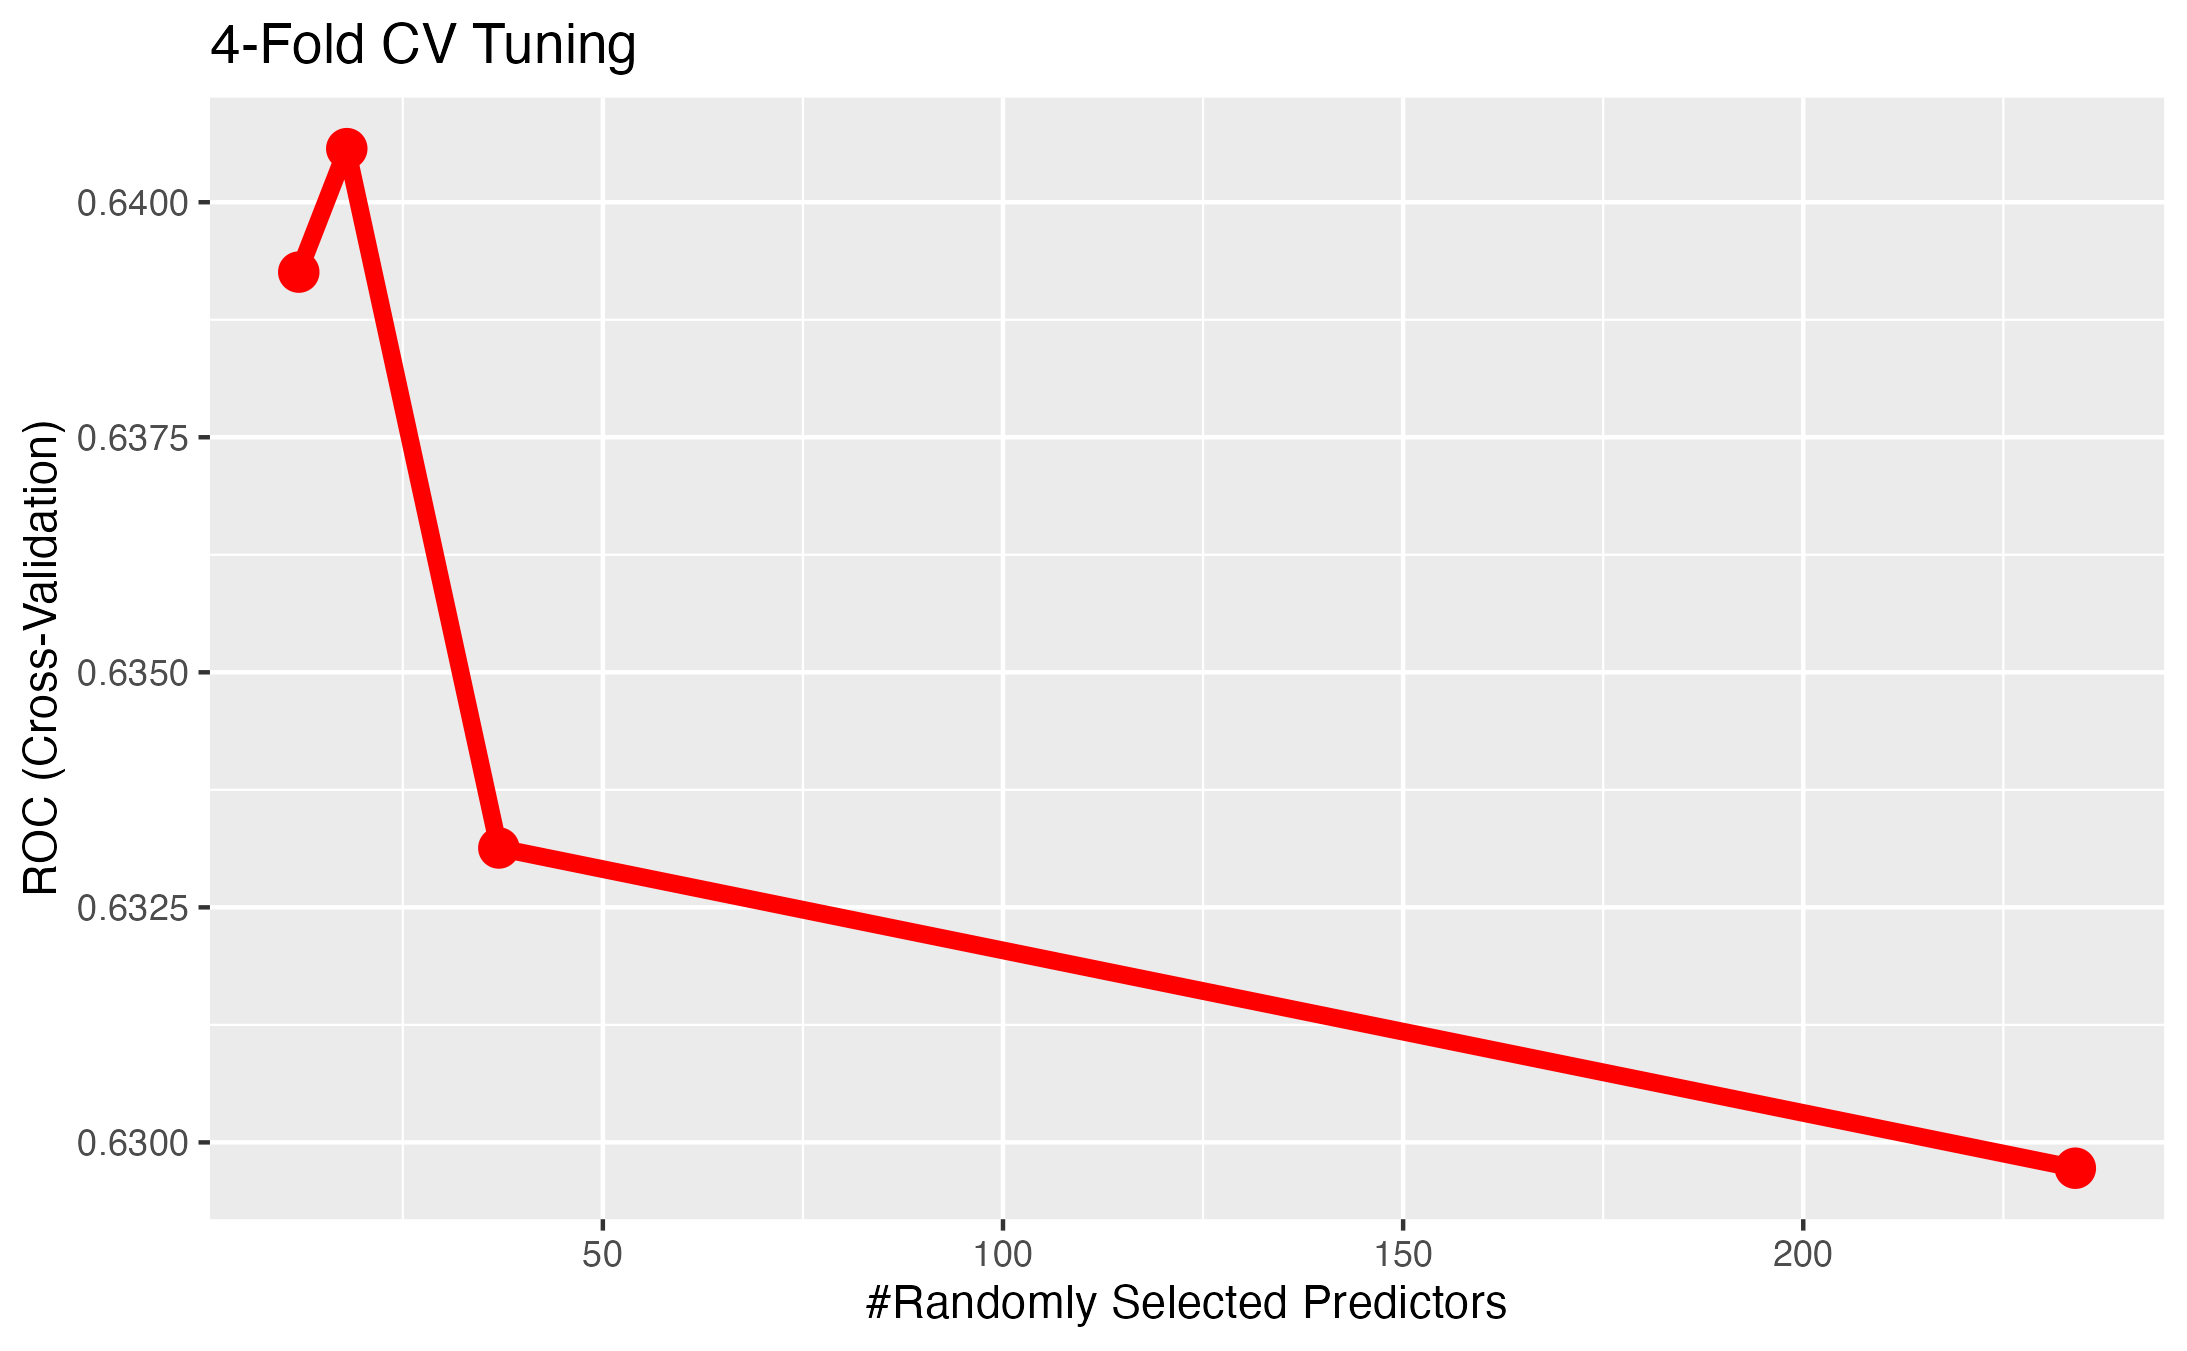
\includegraphics[height=85mm, width=105mm]{desc_cv_rf_tuning.png}
    \caption{Grid Search Tuning Plot for \texttt{mtry} Hyperparameter}
\end{figure}

\


Once the parameters were tuned, the random forest classifier was re-trained using the entire 80\% training data, with a total of $\texttt{n}=500$ trees and $\texttt{mtry}=18$ terms randomly sampled at each split. The training process for this final model took approximately 28 minutes. Using the default 0.5 cut-point, the reported training accuracy was approximately 98\%. This suggests that our model successfully classified the ``good'' rated products from the ``bad'' rated products within our training data, using only the text within their descriptions.

\

Since our model is a classifier, we decided to use a small, randomly selected portion of the test data to determine an optimal cut-point for generating future classifications. Out of the remaining 20\% of unseen text data, we used a 5\% validation set to find the optimal threshold, denoted as $t^{*}$, for making classifications based on the model's predicted probabilities. The remaining 15\% of the data was used for formal testing. We collected performance measures such as \textit{sensitivity}, \textit{specificity}, \textit{balanced-accuracy}, and \textit{accuracy} for different cut points between $t \in (0, 1)$ with a step size of 0.01. Table (7) presents the performance metrics, including only the cut-points that achieved the top 5 accuracy scores on the 5\% validation set. Although the cut-point $t=0.5$ sacrifices specificity for higher sensitivity, we selected $t^{*}=0.5$ as our optimal cut point because it maximizes the overall accuracy on the validation set.


\begin{table}[h!]
    \centering
    \begin{tabular}{| c | c | c | c | c | c |} 
    \hline
    \textbf{Cut-Point ($t$)} &  \textbf{Sensitivity} &  \textbf{Specificity} &  \textbf{Balanced Accuracy} &  \textbf{Accuracy} \\ 
    \hline
    \hline
    0.5 & 0.9214 & 0.1923 & 0.5568 & 0.656 \\
    \hline
    0.55 & 0.8805 & 0.2582 & 0.5694 & 0.654 \\	
    \hline
    0.49 & 0.9214 & 0.1813 & 0.5514 & 0.652	\\
    \hline
    0.51 & 0.9120 & 0.1978 & 0.5549 & 0.652 \\
    \hline
    0.53 & 0.8931 & 0.2308 & 0.5619 & 0.652 \\
    \hline
    \end{tabular}
    \caption{Random Forest Classifier Cut-Point Tuning with Validation Set}
\end{table}

\

The formal testing of our tuned random forest classifier was conducted on a separate test set comprising the remaining 15\% of unseen text data. With the optimal cut-point $t^{*}=0.5$, our model achieved an overall accuracy of approximately 68\%, indicating a successful classification of the ``good'' and ``bad'' ratings for a significant portion of the unseen products. The sensitivity rate was remarkably high at around 94\%, while the specificity rate was significantly lower at approximately 20\%. The resulting confusion matrix is presented in Table (8).

\begin{table}[ht!]
\centering
\begin{tabular}{cc|c|c|c|}
    &\multicolumn{1}{c}{}&\multicolumn{3}{c}{\textbf{Predicted}}\\
    &\multicolumn{1}{c}{}&\multicolumn{1}{c}{\textbf{Bad}}
    &\multicolumn{1}{c}{\textbf{Good}}
    &\multicolumn{1}{c}{\textbf{Total}}\\
    \cline{3-5}
    \multicolumn{1}{c}{\multirow{3}{*}{\rotatebox{90}{\textbf{Actual}}}}
    &\textbf{Bad} &151 & 601 &752\\
    \cline{3-5}
    &\textbf{Good} &78 &1280 & 1358\\
    \cline{3-5}
    &\textbf{Total} &229 & 1881 &\\
    \cline{3-5}
\end{tabular}
\caption{Confusion Matrix for 15\% Testing Data (Using $t^{*}=0.5$)}
\end{table}

\

Considering that our test set contained approximately 64\% positives, the accuracy achieved by our model with the optimal cut-point surpassed the baseline and placed a strong emphasis on the true-positive rate. To assess the predictive performance of our random forest classifier without relying on a fixed cut-point, we also generated the ROC curve depicted in Figure (14).

\begin{figure}[ht!]
    \centering
    \hspace*{-2em}
    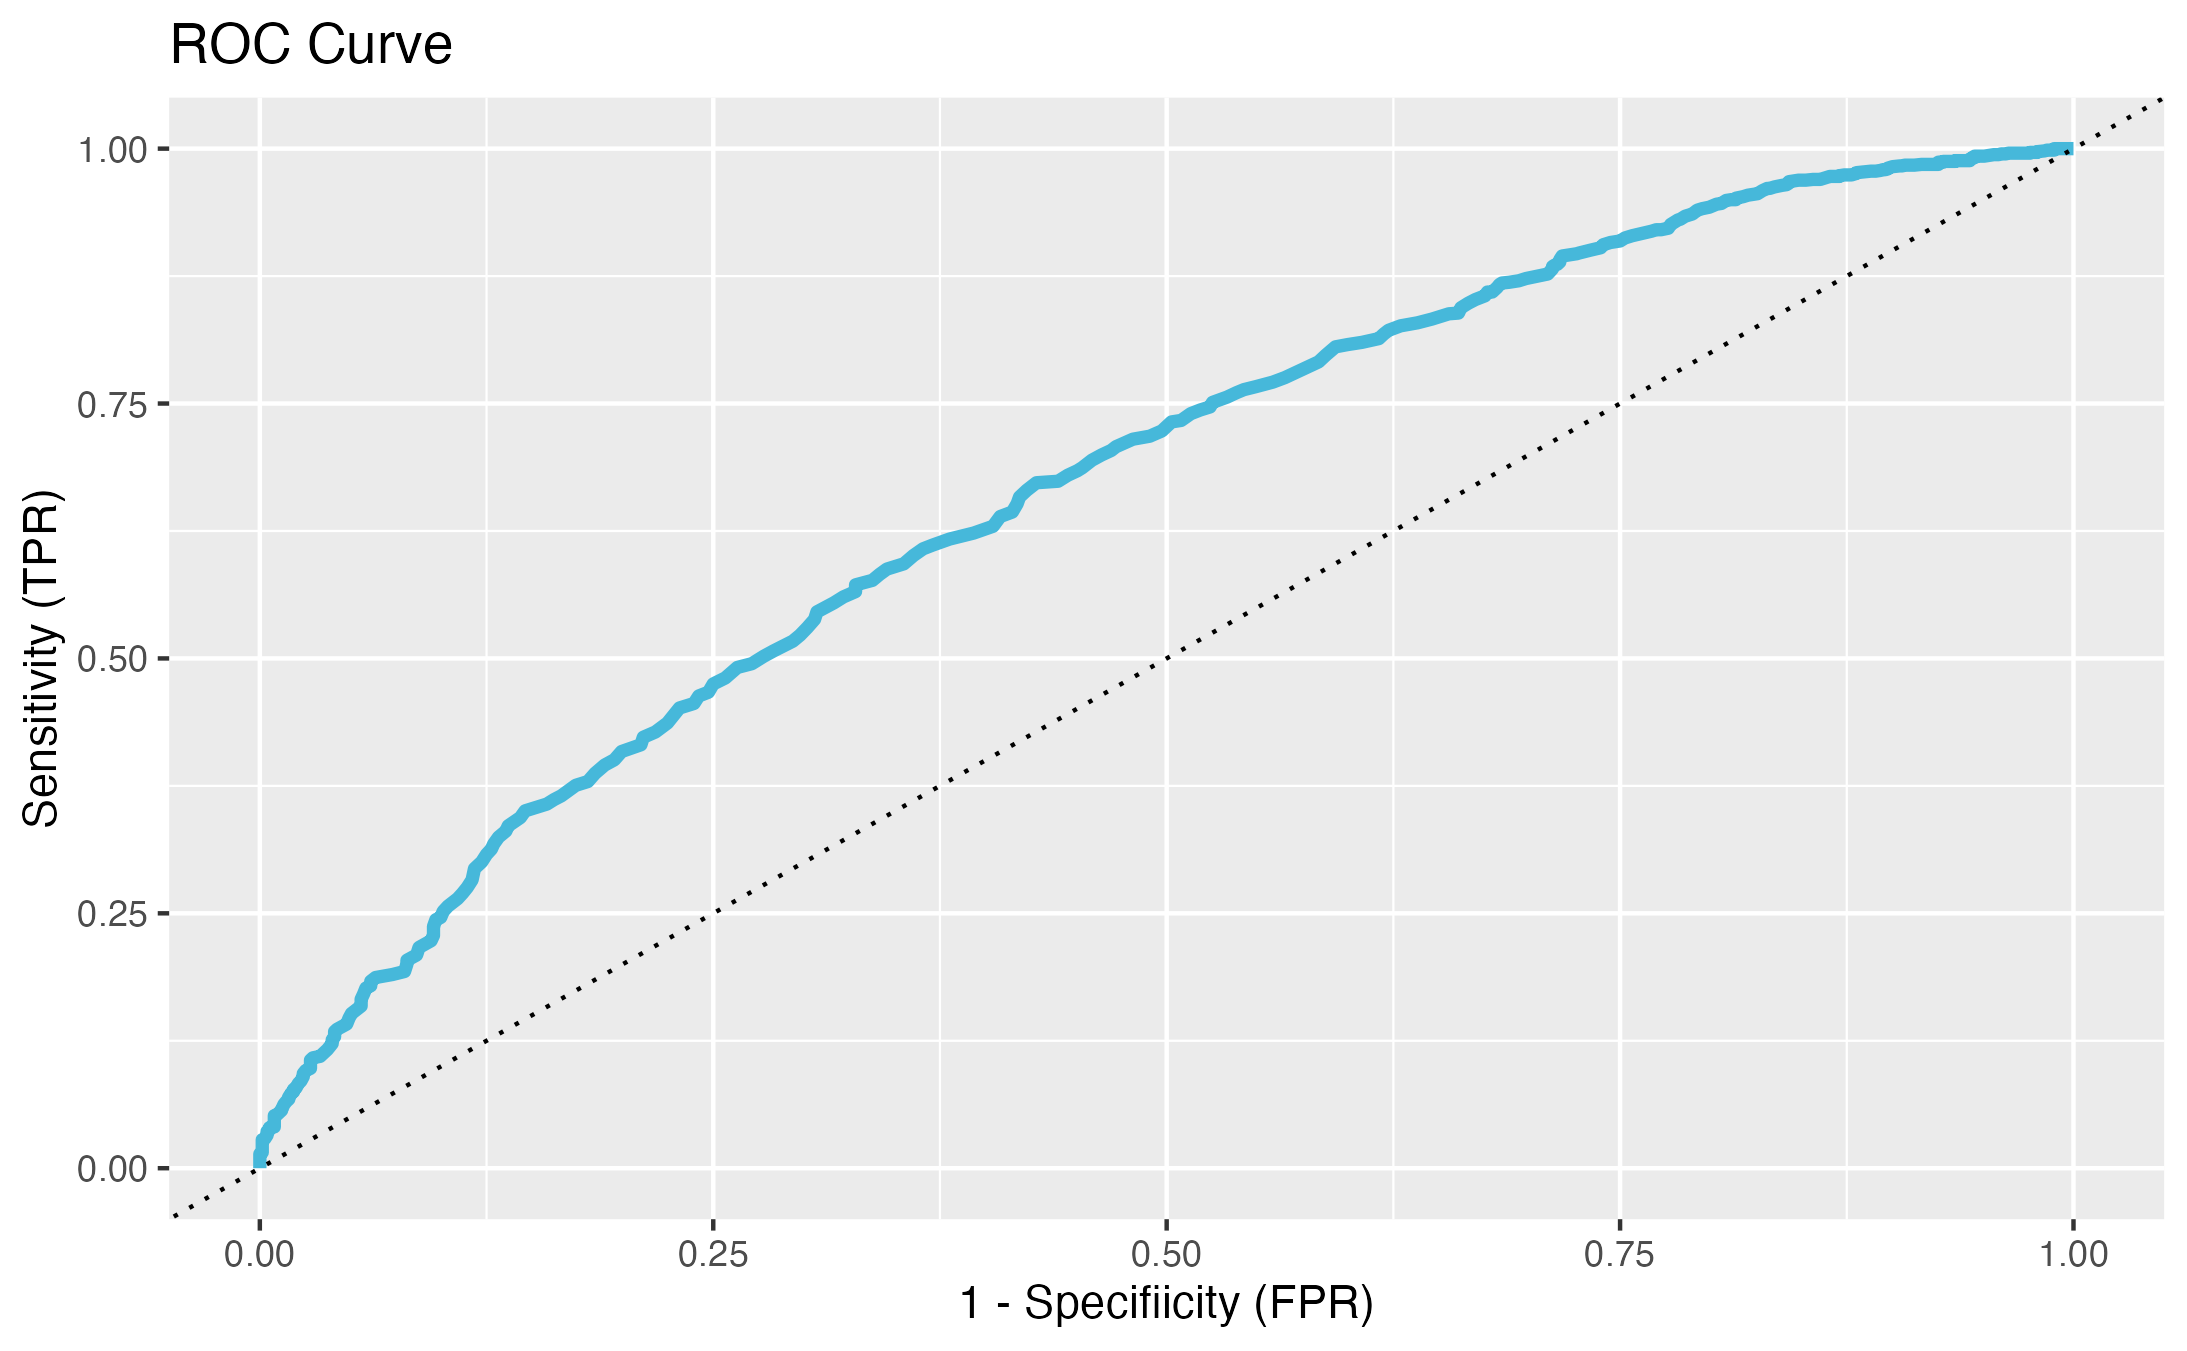
\includegraphics[height=90mm, width=120mm]{desc_results_roc.png}
    \caption{ROC Curve for Random Forest Classifier Using Test Data}
\end{figure}


\

From the ROC curve, we observed a good balance between sensitivity and specificity throughout the range of thresholds. Although the ideal position would be closer to the top-left corner of the plot, the curve demonstrates that our classifier produces significantly better predictions than a random guess (indicated by the black dotted line). The area under the ROC curve in Figure (14) was approximately 0.67, indicating an acceptable discrimination ability of our random forest model in classifying product ratings based on their descriptions.

\


Our trained random forest classifier has exhibited adequate classification performance, prompting us to examine the feature importances generated by the model. Figure (15) showcases the features (or terms) with the highest calculated importance values. The x-axis represents the decrease in the Gini coefficient (\texttt{MeanDecreaseGini}) averaged over the 500 trees. In general, the Gini coefficient assesses how each variable (term) contributes to the homogeneity of the nodes and leaves in the random forest classifier. Therefore, a larger mean decrease in the Gini score indicates a higher importance of the variable (term) in the classifier.

\begin{figure}[ht!]
    \centering
    \hspace*{-2em}
    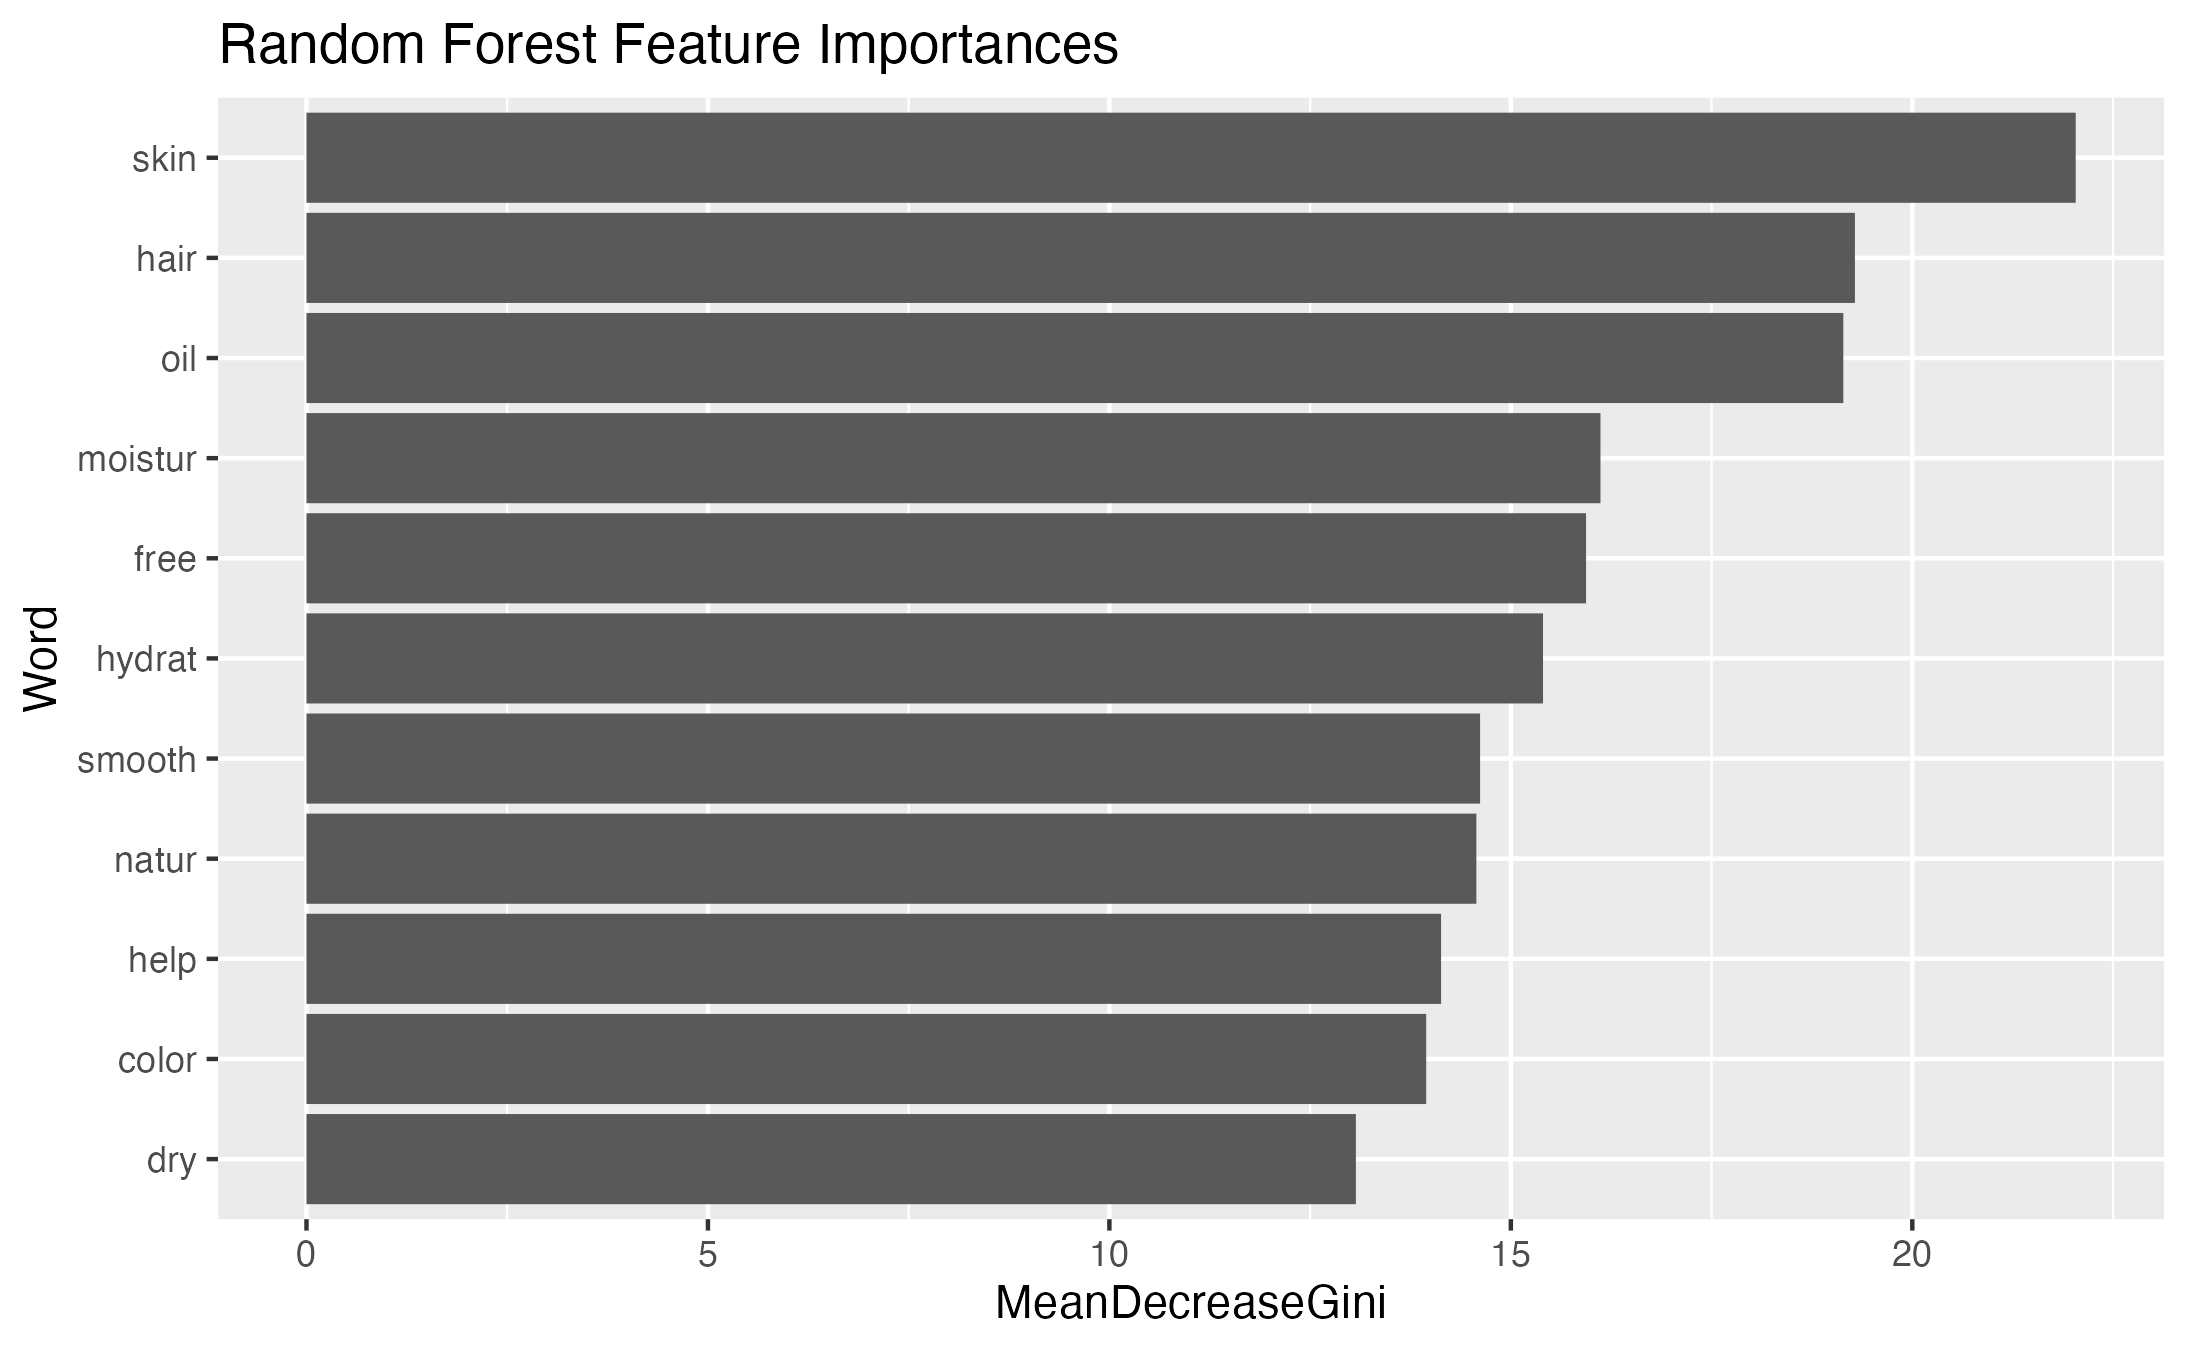
\includegraphics[height=80mm, width=105mm]{desc_feat_imp.png}
    \caption{Feature Importance for the Tuned Random Forest Classifier}
\end{figure}


\

Upon analysis, we observed that terms like ``skin'', ``hair'', and ``oil'' have the most substantial impact on our model's classifications. These terms appear to provide crucial context regarding the product category (e.g., hair care, skin care), which is of utmost importance to our random forest classifier. This finding aligns with the results obtained in Section 3.2, where we discovered a significant relationship between the product category and the product's predicted sentiment. The remaining words depicted in Figure (15) offer similar contextual information, shedding light on which terms from the descriptions had the most influential roles in classifying a product's rating.


\section{Conclusion}

In conclusion, this paper embarked on a comprehensive journey to achieve several distinct goals. Through an exploratory analysis approach, we successfully uncovered customer sentiment at various levels, including individual products, brands, and product categories. Although the predicted sentiment scores were validated using the average star ratings, this analysis provided additional insights into customer perceptions, enabling a deeper understanding of their preferences and sentiments.

\

By delving into product descriptions using tf-idf scores and examining frequently occurring words, we revealed word trends that correlated with the sentiment expressed in \textit{both} customer reviews \textit{and} star ratings. We found that negative sentiment was associated with products related to hair care and eye makeup, while positive sentiment was linked to products related to cleansers and lip \& cheek makeups. Brand and product category analyses based on our \textit{combined rating} scores showed that cologne and fragrance brands received higher ratings, while hair removal and waxing brands received lower ratings. Specific product categories with the highest and lowest ratings were identified for prominent brands, while specific brands with the highest and lowest ratings were identified for popular product categories. This exploration shed light on the language and vocabulary used in the beauty industry, highlighting the significance of specific words in shaping customer perceptions.

\

Furthermore, our implementation of topic modeling allowed us to identify underlying themes and commonalities across diverse brands, offering a holistic view of the beauty industry. This broader perspective provided valuable insights into the shared characteristics and trends within the industry, facilitating comparisons and highlighting unique brand attributes. We ultimately found three major topics within our text data: Topic \#1 pertained to general makeup or lashes, Topic \#2 is associated with facial and body cleansers or moisturizers, and Topic \#3 predominantly relates to hair care.

\

As specific case studies, we provided analyses comparing term frequencies between our derived topics and between chosen makeup brands. These case studies provided examples of insights into the language and characteristics associated with different topics and brands. We found that makeup and skin care products shared common terms in their descriptions, indicating overlap in their language usage. Among the three prominent makeup brands, Colourpop stood out with distinct terms, reflecting a unique brand identity compared to L'Oreal and Maybelline. L'Oreal focused on anti-aging products for slightly older customers, while Colourpop targeted a younger demographic with vibrant and playful descriptors. This analysis revealed the distinctive characteristics and target audiences of different makeup brands based on word frequencies in their product descriptions.

\

In addition to the exploratory analysis, our paper focused on modeling endeavors to formalize the intricate relationships within the Ulta data. We first successfully developed a robust model capable of predicting average star ratings based solely on customer reviews. With additional preprocessing steps performed on our data, a random forest regressor was trained and tuned using a grid search and cross-validation. The final model achieved an RMSE of 0.6176 and an R-Squared of 0.4270 on the test data, indicating good predictive performance. A feature importance plot also revealed that terms such as ``return'', ``disappoint'', and ``love'' had the greatest impact on the model's predictions, aligning with intuitive expectations.

\

Moreover, we unraveled the complex interplay between product price and customer sentiment by modeling their relationship. The analysis was conducted using a binomial logistic regression model with product price as the predictor variable and sentiment as the response variable. The globally fitted model showed that an increase in price corresponds to a more positive sentiment across all product classes and brands. Further analysis at the brand level revealed significant associations between price and sentiment for seven brands, while at the product category level, four categories exhibited a significant relationship. The findings suggest that adjusting prices can influence customer sentiment differently depending on the brand and product category. This analysis provided valuable insights into how price points impact customer perceptions, challenging assumptions and enabling businesses to strategically manage their pricing strategies. 

\

Finally, we leveraged product descriptions to develop a classification model that predicts the general rating of products solely based on their content. After transforming the original star ratings into a categorical variable, we began training a random forest classifier. The classifier was tuned using a grid search with cross-validation, resulting in an optimal choice of hyperparameters. In addition, the model's performance on the test set yielded an overall accuracy of around 68\%, with incredibly high sensitivity. The ROC curve demonstrated acceptable discrimination ability, and an analysis of the feature importances revealed that the most impactful terms for classification were ``skin'', ``hair'', and ``oil''. These findings indicate that specific words in product descriptions may actually be able to explain customer ratings to a certain extent. This text-driven model offers an efficient means of evaluating and assessing products, independent of external factors, empowering both customers and businesses to make informed choices.

\

Overall, this paper significantly enhanced our understanding of the Ulta dataset, uncovering hidden patterns, and providing invaluable insights for consumers and businesses in the beauty industry. The combination of exploratory analysis and focused modeling approaches shed light on the intricate dynamics and trends within Ulta's online store. These findings have practical implications for brands to optimize their strategies, improve customer satisfaction, and foster a deeper understanding of customer preferences. Moving forward, further research can build upon these findings with a larger sample size of reviews for each product to provide a more accurate measure of sentiment.

\end{document}